\documentclass[11pt,a4paper]{article}

% ---- Packages ----
\usepackage[utf8]{inputenc}
\usepackage[T1]{fontenc}
\usepackage{lmodern}
\usepackage[margin=1in]{geometry}
\usepackage{graphicx}
\usepackage{booktabs}
\usepackage{array}
\usepackage{hyperref}
\usepackage{amsmath}
\usepackage{amssymb}
\usepackage{xcolor}
\usepackage{float}
\usepackage{subcaption}
\usepackage{tikz}
\usetikzlibrary{positioning, arrows.meta, shapes.geometric, fit, calc}
\usepackage{listings}

% ---- Listings style ----
\lstset{
  basicstyle=\ttfamily\scriptsize,
  breaklines=true,
  frame=single,
  backgroundcolor=\color{gray!10},
  keywordstyle=\color{blue},
  commentstyle=\color{green!50!black},
  stringstyle=\color{red!70!black},
}

% ---- Custom commands ----
\newcommand{\best}[1]{\textbf{#1}}

% ---- Title ----
\title{
  \vspace{-1cm}
  \LARGE\textbf{Multimodal Presurgical Brain Tumor Classification\\
  Using Statistical Machine Learning}
  \vspace{0.3cm}
}
\author{
  \textbf{Group 12} \\
  STAT3612: Statistical Machine Learning (Spring 2026)
}
\date{}

\begin{document}
\maketitle
\thispagestyle{empty}

\begin{abstract}
This report presents our approach to presurgical brain tumor classification using multimodal data. We design an ensemble system that combines radiology report text (via BioClinicalBERT and TF-IDF), clinical features (signal intensity patterns, tumor location), and MRI-derived features (ResNet-50 embeddings with per-modality PCA) to classify brain tumors into five types: Glioma, Meningioma, Brain Metastase, Sellar region tumors, and Pineal/Choroid Plexus tumors.

Our design is guided by a systematic analysis of each data modality's discriminative power. We find that radiology reports alone achieve $\sim$84\% Micro-F1 and provide the dominant signal, while clinical features ($\sim$67\%), image features ($\sim$57\%), and raw radiomic features ($\sim$52\%, near random) contribute progressively less. Based on this analysis, we design a dual-path neural network where BioClinicalBERT processes report text and a tabular encoder handles clinical and location features, connected by a cross-modal gate that adaptively controls information flow between paths. We complement this with three gradient-boosted tree models (XGBoost, LightGBM, CatBoost) trained on TF-IDF report features combined with clinical data. The final 6-model weighted ensemble achieves \best{87.25\%} out-of-fold Micro-F1 on 2,266 training samples across 5-fold cross-validation.

A central challenge is the potential for distribution shift between training and test sets. We employ NN-dominant ensemble weighting and hierarchical location encoding as potential mitigation strategies, and note that OOF estimates may be optimistic if test distributions differ from training.
\end{abstract}

\tableofcontents
\newpage

% ============================================================
% SECTION 1: Introduction
% ============================================================
\section{Introduction}
\label{sec:intro}

Accurate presurgical diagnosis of brain tumors is essential for treatment planning and patient management. Different tumor types require substantially different therapeutic strategies---gliomas may necessitate maximal safe surgical resection, meningiomas are often managed with surgery or observation, while brain metastases may be treated with radiation therapy or targeted systemic treatment~\cite{price2024}. A reliable, automated preoperative classification system can thus play an important role in supporting clinical decision-making and improving patient outcomes.

Magnetic Resonance Imaging (MRI) is the primary imaging modality used for brain tumor diagnosis and monitoring~\cite{wang2024}. In clinical practice, radiologists interpret multi-sequence MRI findings together with patient demographics and summarize their assessment in radiology reports. However, manual interpretation is challenged by overlapping imaging characteristics across tumor types, inter-observer variability, and the complexity of integrating information from multiple modalities. This motivates the development of machine learning models that can systematically combine multimodal data for tumor classification.

In this project, we address the task of five-class brain tumor classification using multimodal data comprising radiology reports, MRI-derived features, and clinical information. The classification task presents several fundamental challenges:

\begin{itemize}
  \item \textbf{Severe class imbalance:} Gliomas account for nearly half of all cases (46.6\%), while Pineal/Choroid Plexus tumors constitute only 1.1\%, creating a 40:1 imbalance ratio that biases models toward majority classes.
  \item \textbf{Multimodal integration:} Diagnostic information is spread across modalities with fundamentally different statistical properties---unstructured text (radiology reports), high-dimensional continuous features (image embeddings), categorical variables (signal intensity patterns), and tabular data (demographics)---requiring careful fusion strategies.
  \item \textbf{Distribution shift:} The test set may exhibit systematic differences from training data in feature distributions, missing data patterns, and location vocabulary. Standard cross-validation estimates may be overly optimistic under such covariate shift, motivating the use of robustness-promoting strategies throughout our design.
  \item \textbf{Limited sample size:} With only 2,266 training samples and feature dimensions up to 8,192 (raw image features), there is a severe risk of overfitting that demands aggressive dimensionality reduction and regularization.
\end{itemize}

Our approach is guided by a principled analysis of what each data modality contributes. Before designing any model, we first measure the solo discriminative power of each source through 5-fold cross-validation: radiology reports ($\sim$84\% Micro-F1), clinical features ($\sim$67\%), image features ($\sim$57\%), and raw radiomic features ($\sim$52\%, near the 46.6\% majority-class baseline). This ranking directly informs our architecture---we allocate the most capacity to the strongest signal (reports) and remove modalities that add noise (raw radiomics, shifted image features in the neural network).

Based on this analysis, we design a multimodal ensemble system with the following key components:

\begin{enumerate}
  \item \textbf{Dual-path neural network with cross-modal gating.} Path A encodes radiology reports using BioClinicalBERT~\cite{alsentzer2019} (fine-tuning the top 2 layers). Path B encodes tabular features (clinical data, signal intensity patterns, tumor location with hierarchical parsing). A learned gate controls how much cross-modal information to inject, allowing the model to rely on reports when they are informative and supplement with tabular data when reports are ambiguous.
  \item \textbf{Tree-based models on report and clinical features.} Three gradient-boosted tree models (XGBoost~\cite{chen2016}, LightGBM~\cite{ke2017}, CatBoost~\cite{prokhorenkova2018}) are trained on TF-IDF vectorized report text combined with clinical and location features. These models capture different decision boundary patterns from the neural network, providing ensemble diversity.
  \item \textbf{Weighted probability ensemble.} A grid search over OOF predictions determines optimal blend weights across all 6 models, finding NN=40\% and MLU=60\% as optimal. The final ensemble achieves \best{87.25\%} out-of-fold Micro-F1 with grid-search weights, and 86.98\% with the submission configuration.
\end{enumerate}

The remainder of this report is organized as follows. Section~\ref{sec:dataset} describes the dataset and exploratory data analysis. Section~\ref{sec:method} presents our methodology, including feature engineering, model architecture design, and ensemble strategy, with emphasis on \emph{why} each design choice was made. Section~\ref{sec:experiments} details experiments and results with ablation studies. Section~\ref{sec:discussion} discusses key findings, challenges, and lessons learned. Section~\ref{sec:conclusion} concludes with future directions.


% ============================================================
% SECTION 2: Dataset & EDA
% ============================================================
\section{Dataset and Exploratory Data Analysis}
\label{sec:dataset}

\subsection{Dataset Overview}

The dataset comprises patients with brain tumors, divided into training (1,983), validation (283), and test (378) splits. Each patient is associated with five data modalities: MRI-derived features (radiomics and deep image features), radiology reports, and clinical/demographic information. The task is five-class classification into Glioma, Meningioma, Brain Metastase Tumour, Tumors of the Sellar Region, and Pineal Tumour / Choroid Plexus Tumour.

For our final pipeline, we merge the training and validation sets (2,266 samples) and use 5-fold stratified cross-validation for model selection and out-of-fold (OOF) evaluation. Predictions are generated on an independent new test set of 378 samples (released after the original test set was found to contain case ID leakage with the training data).

\subsection{Class Distribution}

\begin{figure}[H]
\centering
% FIGURE: Class Distribution Bar Chart
% Generate: figures/class_distribution.png
%
% Chart type: Horizontal bar chart
% Data (5 bars, sorted by count descending):
%   Glioma                                    = 1056 (46.6%)  ← steelblue
%   Meningioma                                = 832  (36.7%)  ← steelblue
%   Brain Metastase Tumour                    = 288  (12.7%)  ← steelblue
%   Tumors of the sellar region               = 64   (2.8%)   ← coral (minority)
%   Pineal tumour and Choroid plexus tumour   = 26   (1.1%)   ← coral (minority)
%
% Annotations:
%   - Show count AND percentage at end of each bar (e.g., "1056 (46.6%)")
%   - Add a vertical dashed line at 1056 labeled "Majority baseline (46.6%)"
%   - Highlight minority classes (Sellar + Pineal) in coral
%   - Title: "Class Distribution (Train + Val, N=2,266)"
%   - X-axis: "Count"   Y-axis: class names
%   - Use figure size (10, 4), tight layout
%   - Light gray grid lines on x-axis
%
% Data source: model_final.ipynb Cell 4
%
\includegraphics[width=0.8\textwidth]{figures/class_distribution.png}
\caption{Class distribution of brain tumor types in the training and validation sets (N=2,266). Minority classes (Sellar, Pineal/CP) are highlighted in coral.}
\label{fig:class_distribution}
\end{figure}

\begin{table}[H]
\centering
\caption{Class distribution across dataset splits.}
\label{tab:class_dist}
\begin{tabular}{lrrrr}
\toprule
\textbf{Class} & \textbf{Train} & \textbf{Val} & \textbf{Total} & \textbf{Proportion} \\
\midrule
Glioma & 924 & 132 & 1,056 & 46.6\% \\
Meningioma & 728 & 104 & 832 & 36.7\% \\
Brain Metastase & 252 & 36 & 288 & 12.7\% \\
Sellar Region & 56 & 8 & 64 & 2.8\% \\
Pineal / CP & 23 & 3 & 26 & 1.1\% \\
\midrule
\textbf{Total} & 1,983 & 283 & 2,266 & 100\% \\
\bottomrule
\end{tabular}
\end{table}

The dataset exhibits severe class imbalance with a 40:1 ratio between the majority class (Glioma, 46.6\%) and the rarest class (Pineal/CP, 1.1\%). A naive majority-class classifier would achieve 46.6\% Micro-F1, establishing a lower bound that raw radiomic features barely exceed. This imbalance has two important consequences: (1) overall Micro-F1 is dominated by performance on Glioma and Meningioma (83.3\% of data), and (2) minority class performance (especially Pineal/CP with only 26 samples) requires special handling.

\subsection{Data Modalities}
\label{sec:modalities}

Each patient sample includes data from five distinct sources. Table~\ref{tab:modalities} summarizes their characteristics and standalone predictive power, measured via 5-fold cross-validation on the training set.

\begin{table}[H]
\centering
\caption{Summary of available data modalities and their standalone Micro-F1 performance (5-fold CV).}
\label{tab:modalities}
\begin{tabular}{llrcl}
\toprule
\textbf{Modality} & \textbf{Encoding} & \textbf{Dim} & \textbf{Solo F1} & \textbf{Role} \\
\midrule
Radiology Report & TF-IDF + SVD-64 & 64 & 84.29\% & Primary signal \\
Clinical + SI & One-hot + numeric & 27 & 66.51\% & Complementary \\
Location & Label-encoded + LGB & 1 & 62.67\% & Moderate proxy \\
Image (ResNet) & Per-mod PCA & 128 & 56.97\% & Weak, shifted \\
Radiomics (raw) & Numeric & 20 & 52.21\% & Near random \\
\bottomrule
\end{tabular}
\end{table}

\begin{figure}[H]
\centering
% FIGURE: Solo Modality Performance
% Generate: figures/solo_modality_performance.png
%
% Chart type: Horizontal bar chart
% Data (5 bars, sorted by F1 descending):
%   Radiology Report (TF-IDF+SVD-64) = 84.29%  ← #2196F3 (blue, strong)
%   Clinical + SI (27d)                  = 66.51%  ← color: #4CAF50 (green, moderate)
%   Location (label-encoded, 1d)         = 62.67%  ← color: #4CAF50 (green, moderate)
%   Image (per-mod PCA, 128d)            = 56.97%  ← color: #FF9800 (orange, weak)
%   Radiomics (raw, 20d)                 = 52.21%  ← color: #F44336 (red, near-random)
%
% Reference line: Vertical dashed line at x=46.6% labeled "Majority-class baseline (46.6%)"
%
% Annotations:
%   - Show percentage at end of each bar (e.g., "84.29%")
%   - Show dimension in parentheses after modality name (e.g., "Radiology Report (64d)")
%   - Title: "Solo Modality Performance (5-Fold CV, Micro-F1)"
%   - X-axis: "Micro-F1 (%)"   Y-axis: modality names
%   - Use figure size (10, 4), tight layout
%   - Light gray grid lines on x-axis
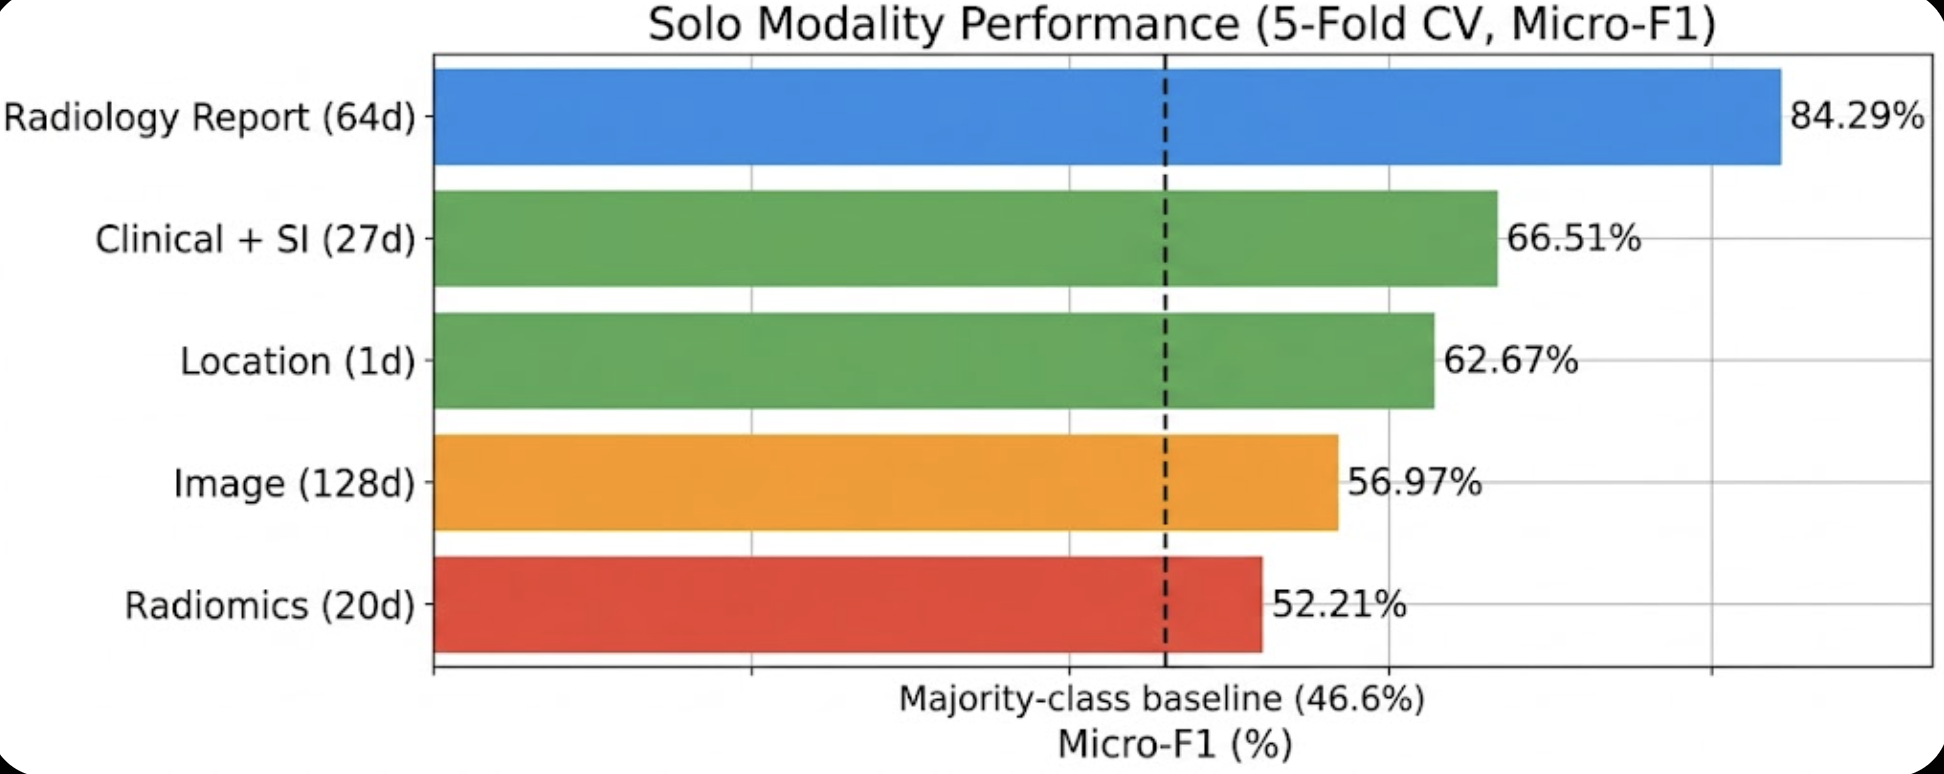
\includegraphics[width=0.8\textwidth]{figures/solo_modality_performance.png}
\caption{Standalone Micro-F1 performance of each data modality (5-fold CV). The dashed line indicates the majority-class baseline (46.6\%). Color encodes discriminative strength: blue (strong), green (moderate), orange (weak), red (near-random).}
\label{fig:solo_modality}
\end{figure}

The most striking finding is the gap between reports ($\sim$84\%) and all other modalities. Radiology reports encode the radiologist's full diagnostic reasoning---location, enhancement patterns, edema characteristics---making them the single most informative feature. All other modalities provide diminishing complementary value.

\subsubsection{Radiology Reports}

Each patient has a radiologist-written report describing the MRI findings. Importantly, only the findings section is provided; the impression section is excluded to prevent direct diagnostic label leakage. These reports encode the most clinically relevant diagnostic features: tumor location, enhancement patterns, edema characteristics, and morphological descriptions.

We process reports via two approaches: (1) TF-IDF vectorization (max 8,000 features, trigrams) with truncated SVD (64--256 dimensions depending on model; 64 for solo evaluation, 256 for MLU tree models), and (2) BioClinicalBERT~\cite{alsentzer2019} with fine-tuning of the top 2 layers (frozen embeddings yield $\sim$82\% solo, fine-tuning improves generalization). Using TF-IDF+SVD-64 alone, reports achieve 84.29\% Micro-F1, making them by far the strongest single modality.

\subsubsection{Clinical and Signal Intensity Features}

Clinical data includes patient demographics and features extracted from the radiology reports by the data providers:

\begin{itemize}
  \item \textbf{Demographics:} Age (numeric, $\sim$70\% missing) and Sex (categorical, $\sim$70\% unknown). Age is imputed with the training median and augmented with a binary missing flag.
  \item \textbf{Signal Intensity (SI) patterns:} One-hot encoded descriptions of MRI signal characteristics across four modalities (T1, T1c, T2, T2-FLAIR). Each modality has 6 possible values (hypointense, isointense, hyperintense, heterogeneous, homogeneous, unknown), yielding 24 binary features. These patterns encode enhancement and heterogeneity---key diagnostic markers.
  \item \textbf{Tumor location:} A categorical feature with 719 unique anatomical labels in train+val. Examples include ``frontal lobe,'' ``cerebellopontine angle.'' Location is a strong proxy for tumor type (e.g., sellar region tumors are almost always of the Sellar class). We use both a learned embedding (10 dimensions in the neural network) and NLP-based hierarchical parsing (region, hemisphere, lobe) for robustness to unseen locations.
\end{itemize}

Combined Clinical + SI features achieve 66.51\% Micro-F1 alone. Location alone (label-encoded, 1 dimension) achieves 62.67\%. When Clinical + SI + Location are combined with NLP-parsed location features, the tabular features reach up to 79.83\% Micro-F1, demonstrating that location is the key secondary signal after reports.

\subsubsection{Cross-Modal Radiomic Ratios}

A central finding of our analysis is that \emph{raw radiomic features are near-random ($\sim$52\%), but cross-modal ratios derived from them can be informative when combined with other features}. This has a clear clinical explanation. Radiologists do not diagnose tumors by looking at texture statistics in isolation---they compare signal intensity \emph{across MRI sequences}. For example:
\begin{itemize}
  \item A tumor that is \textbf{bright on T1c but dark on T1} (high T1c/T1 ratio) shows contrast enhancement, suggesting blood-brain barrier disruption---common in high-grade gliomas and metastases.
  \item A tumor with \textbf{high T2-FLAIR but moderate T2} (high T2F/T2 ratio) shows surrounding vasogenic edema---typical of metastases and meningiomas.
\end{itemize}

The five raw PyRadiomics features per modality (Mean, Entropy, 90th Percentile, GLCM Contrast, GLCM Joint Entropy) measure absolute texture statistics. These values alone do not distinguish tumor types. We compute \emph{ratios across modalities} for the same feature to recover cross-sequence contrasts. Table~\ref{tab:ratios} summarizes the engineered ratios:

\begin{table}[H]
\centering
\caption{Engineered cross-modal ratio features and their clinical significance.}
\label{tab:ratios}
\begin{tabular}{lll}
\toprule
\textbf{Ratio} & \textbf{Formula} & \textbf{Clinical Significance} \\
\midrule
Enhancement & T1c / T1 & Contrast enhancement (BBB disruption) \\
Edema & T2F / T2 & Edema pattern (vasogenic vs.\ infiltrative) \\
Tissue contrast & T1 / T2 & Tissue composition (fat, blood, calcification) \\
$\Delta$ Enhancement & T1c $-$ T1 & Absolute enhancement magnitude \\
$\Delta$ Edema & T2F $-$ T2 & Absolute edema extent \\
\bottomrule
\end{tabular}
\end{table}

Each ratio is computed for all 5 radiomic features (25 total), log-transformed (clipped to [0.01, 100]), and augmented with 4 per-modality missing flags. However, experiments show these ratios alone still achieve only $\sim$52\%---they do not add discriminative power independently. We include them in the neural network's tabular path because they are computationally free and encode domain knowledge, but their contribution to final performance is marginal.

\subsubsection{Deep Image Features}

Deep image features are extracted from ResNet-50~\cite{he2016} applied to representative 2D MRI slices across four modalities (T1, T1c, T2, T2-FLAIR), yielding 2,048 features per modality (8,192 total). We apply \textbf{per-modality PCA} (128 dimensions each, fit on training data only, explaining 94.16\% of variance) for a final 512-dimensional image representation.

\textbf{Why per-modality PCA over mean-pooling:} Mean-pooling across modalities destroys complementary physical information. T1 and T1-contrast capture anatomy and vascularity, while T2 and T2-FLAIR capture edema patterns. Per-modality PCA preserves each sequence's unique diagnostic signal, resulting in a sample-to-feature ratio of $\sim$4.4:1 (2,266 samples / 512 features) versus $\sim$0.28:1 without PCA.

Despite PCA, image features achieve only 56.97\% Micro-F1 solo and suffer from distribution shift between training and test sets (Section~\ref{sec:shift}). We include them in tree models (ImgTab) but exclude them from the neural network path to avoid injecting shifted features.

\subsubsection{Radiomic Features}

Five PyRadiomics features are extracted per MRI modality: Mean, Entropy, 90th Percentile, GLCM Contrast, and GLCM Joint Entropy (20 features total). These global texture statistics carry near-zero discriminative power (52.21\% Micro-F1, barely above the 46.6\% majority-class baseline). This is expected because these features capture aggregate texture statistics rather than the clinically relevant patterns (location, enhancement, edema) that drive radiologist diagnosis.

\subsection{Missing Data Patterns}

Missing data is prevalent and non-random across modalities:

\begin{table}[H]
\centering
\caption{Missing data patterns in training data and handling strategies.}
\label{tab:missing}
\begin{tabular}{lrl}
\toprule
\textbf{Feature} & \textbf{Missing Rate} & \textbf{Handling} \\
\midrule
Age & 70.1\% & Median imputation + binary missing flag \\
Sex & 70.1\% & ``Unknown'' as separate category \\
T1 radiomics & 0.1\% & Zero-filled + per-modality missing flag \\
T1c radiomics & 31.3\% & Zero-filled + per-modality missing flag \\
T2 radiomics & 30.9\% & Zero-filled + per-modality missing flag \\
T2F radiomics & 36.1\% & Zero-filled + per-modality missing flag \\
Location & 0\% & Always available \\
Report & 0\% & Always available \\
\bottomrule
\end{tabular}
\end{table}

The high missing rate for demographics ($\sim$70\%) limits their standalone value, but the missingness pattern itself is an informative signal, making missing flags useful features.

\subsection{Robustness Considerations}
\label{sec:shift}

A practical concern in deploying any clinical classifier is robustness to distribution shift---changes in patient demographics, imaging protocols, or reporting styles between training and deployment. Our system incorporates several design choices that promote generalization without requiring access to test data:

\begin{enumerate}
  \item \textbf{High missingness rates in training data} ($\sim$70\% for Age and Sex, 31--36\% for T1c/T2/T2F radiomics). We treat missingness as an informative feature (binary missing flags) rather than a nuisance, which makes the model robust to variations in data completeness at deployment time.
  \item \textbf{Large location vocabulary} (719 unique anatomical labels in training). Many locations appear only once or twice, so we use hierarchical parsing (region/hemisphere/lobe) that decomposes even novel anatomical descriptions into known categories.
  \item \textbf{BERT semantic embeddings} represent clinical meaning (``ring-enhancing lesion'' = vascular tumor) rather than surface word frequencies, making the report encoder more robust to vocabulary changes than TF-IDF-based approaches.
  \item \textbf{Ensemble diversity} across fundamentally different input signals (BERT text, TF-IDF tabular, NN probabilities, image features) ensures that no single model's failure mode dominates predictions.
\end{enumerate}

These strategies are standard approaches for building robust models. We note that the effectiveness of any robustness strategy cannot be confirmed without labeled out-of-distribution data, and our OOF cross-validation estimates may be optimistic if the deployment distribution differs substantially from training.


% ============================================================
% SECTION 3: Methodology
% ============================================================
\section{Methodology}
\label{sec:method}

Our system has four components: (1) feature engineering, (2) a dual-path neural network with cross-modal gating, (3) gradient-boosted tree models, and (4) a weighted probability ensemble.

\begin{figure}[H]
\centering
% FIGURE: System Overview — REGENERATE NEEDED (update weights and OOF)
% Generate: figures/system_overview.png
%
% Layout: Left-to-right flow, 3 columns:
%
% Column 1 (Data Sources) — 3 rounded boxes stacked:
%   "Radiology Report" (blue border)
%   "Clinical + SI + Location" (green border)
%   "Image Features (PCA)" (gray border, label "inactive in NN" in small text)
%
% Column 2 (Models) — 3 rounded boxes:
%   "Neural Network" with subtitle "BERT + Tabular + CrossModalGate"
%   "MLU Models" with subtitle "XGB + LGB + CB"
%   "Auxiliary" with subtitle "NNXGB (NN probs→XGB) + ImgTab"
%
% Column 3 (Ensemble) — 1 box:
%   "Weighted Blend" with subtitle "87.25% OOF"
%
% Arrows:
%   Report → Neural Network (blue)
%   Report → MLU Models (blue)
%   Clinical+SI+Location → Neural Network (green)
%   Clinical+SI+Location → MLU Models (green)
%   Clinical+SI+Location → Auxiliary (green)
%   Image → Auxiliary (gray, dashed)
%   All 3 model boxes → "Weighted Blend"
%
% Below "Weighted Blend" box, show weights (submission config):
%   NN: 40%  |  MLU_XGB: 30%  |  MLU_LGB: 30%  |  MLU_CB: 0%  |  NNXGB: 5%  |  ImgTab: 5%  (grid-search optimal)
%
% Style: Clean, white background, rounded corners, no internal details.
% Figure size: (12, 5), tight layout
%
% Data source: model_final.ipynb Cell 25
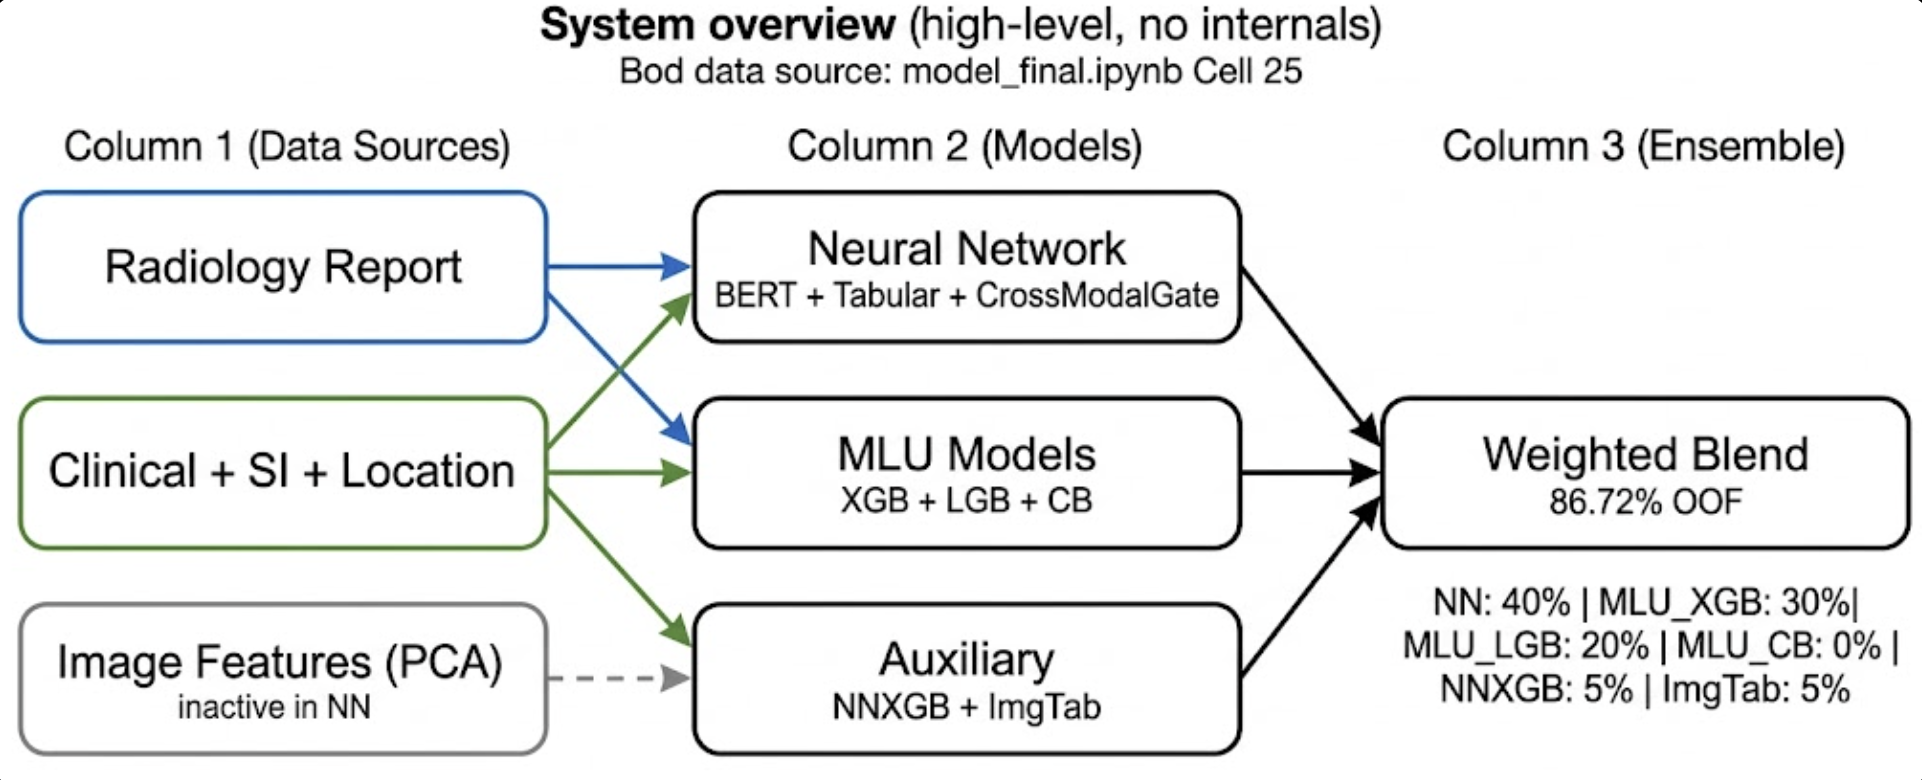
\includegraphics[width=\textwidth]{figures/system_overview.png}
\caption{System overview. Radiology reports and clinical features feed into both neural network and tree models. NNXGB uses the NN's 5-d class probabilities as input features for XGBoost. The image path is used only in the ImgTab auxiliary model (dashed arrow). All 6 model probabilities are combined via weighted blend achieving 87.25\% OOF Micro-F1.}
\label{fig:system_overview}
\end{figure}

\subsection{Feature Engineering}
\label{sec:feat_eng}

Our preprocessing mirrors how radiologists read scans: they compare across MRI sequences, combine findings with anatomical location, and consider patient demographics. Table~\ref{tab:feature_summary} summarizes all features.

\begin{table}[H]
\centering
\caption{Summary of engineered features.}
\label{tab:feature_summary}
\begin{tabular}{llcl}
\toprule
\textbf{Source} & \textbf{Encoding} & \textbf{Dim} & \textbf{Used By} \\
\midrule
Report (TF-IDF+SVD) & Trigram TF-IDF $\to$ SVD-256 & 256 & MLU tree models \\
Report (BERT) & BioClinicalBERT CLS token & 768 & Neural network \\
Demographics & Sex, Age, Age\_missing & 3 & NN tabular + ImgTab \\
Signal Intensity & One-hot, 6 values $\times$ 4 modalities & 24 & NN tabular + ImgTab \\
Location (label) & Learned embedding & 10 & NN tabular \\
Location (hierarchy) & Region + hemisphere + lobe & 3 & NN tabular + MLU \\
Cross-modal Ratios & Log ratios across modalities & 25 & NN tabular + MLU \\
Missing flags & Per-modality radiomics & 4 & NN tabular \\
SI Unknown ratio & Fraction of unknown SI & 1 & MLU \\
Image (PCA) & Per-modality PCA & 512 & ImgTab \\
\bottomrule
\end{tabular}
\end{table}

\textbf{Key design choices:}

\begin{itemize}
  \item \textbf{Location has two representations:} A label-encoded index (for the NN embedding) and a hierarchical parse into region/hemisphere/lobe (3 features). The hierarchy handles novel test locations---even if ``left posterior frontal gyrus'' is unseen, we extract region=brain, hemisphere=left, lobe=frontal.
  \item \textbf{Cross-modal ratios:} We compute T1c/T1 (enhancement), T2F/T2 (edema), T1/T2 (tissue contrast), and their deltas for each of 5 radiomic features (25 total). These transform absolute texture statistics into clinically meaningful relative contrasts. However, experiments show these ratios alone remain near-random ($\sim$52\%); we include them as they encode domain knowledge at zero cost.
  \item \textbf{Per-modality PCA for images:} Mean-pooling destroys complementary physical information (T1/T1c = anatomy/vascularity; T2/T2F = edema). Per-modality PCA (128d each, 94.16\% variance explained) preserves each sequence's diagnostic signal.
\end{itemize}

\subsection{Dual-Path Neural Network}
\label{sec:nn}

\textbf{Why dual-path, not unified transformer?} Our initial architecture (v1) used a 6-token transformer giving equal weight to all modalities. It failed ($\sim$80\%) because weak modalities (image $\sim$57\%, radiomics $\sim$52\%) dragged down the strong ones (report $\sim$84\%). The dual-path design isolates each modality's encoding so weak features cannot contaminate strong ones.

\subsubsection{Report Encoder}

\begin{figure}[H]
\centering
% FIGURE: Report Encoder Detail
% Generate: figures/report_encoder.png
%
% Layout: Vertical flow diagram
%
% [Input: Token IDs, shape (128,)]  ← show as small box
%          ↓
% [BioClinicalBERT]  ← large box, split into two sections:
%   Top section: "Layers 0–9 (frozen)" — gray background, padlock icon
%   Bottom section: "Layers 10–11 (fine-tuned)" — blue background
%          ↓
% [CLS token, 768d]  ← small box
%          ↓ fork into two branches side by side:
%
%   Left branch:                    Right branch:
%   [Linear 768→288]               [Linear 768→288]
%   [LayerNorm → GELU]             (no activation, just linear)
%   [Dropout 0.15]
%        ↓                              ↓
%   proj_out (288d)               residual (288d)
%        ↓────────── + ──────────────↓
%                   ↓
%             report_emb (288d)
%
% Annotations:
%   - Mark "768d" and "288d" on arrows
%   - Label the sum node as "residual connection"
%   - Show "Dropout 0.15" only on left branch
%
% Figure size: (10, 6), clean style
%
% Data source: model_final.ipynb Cell 14
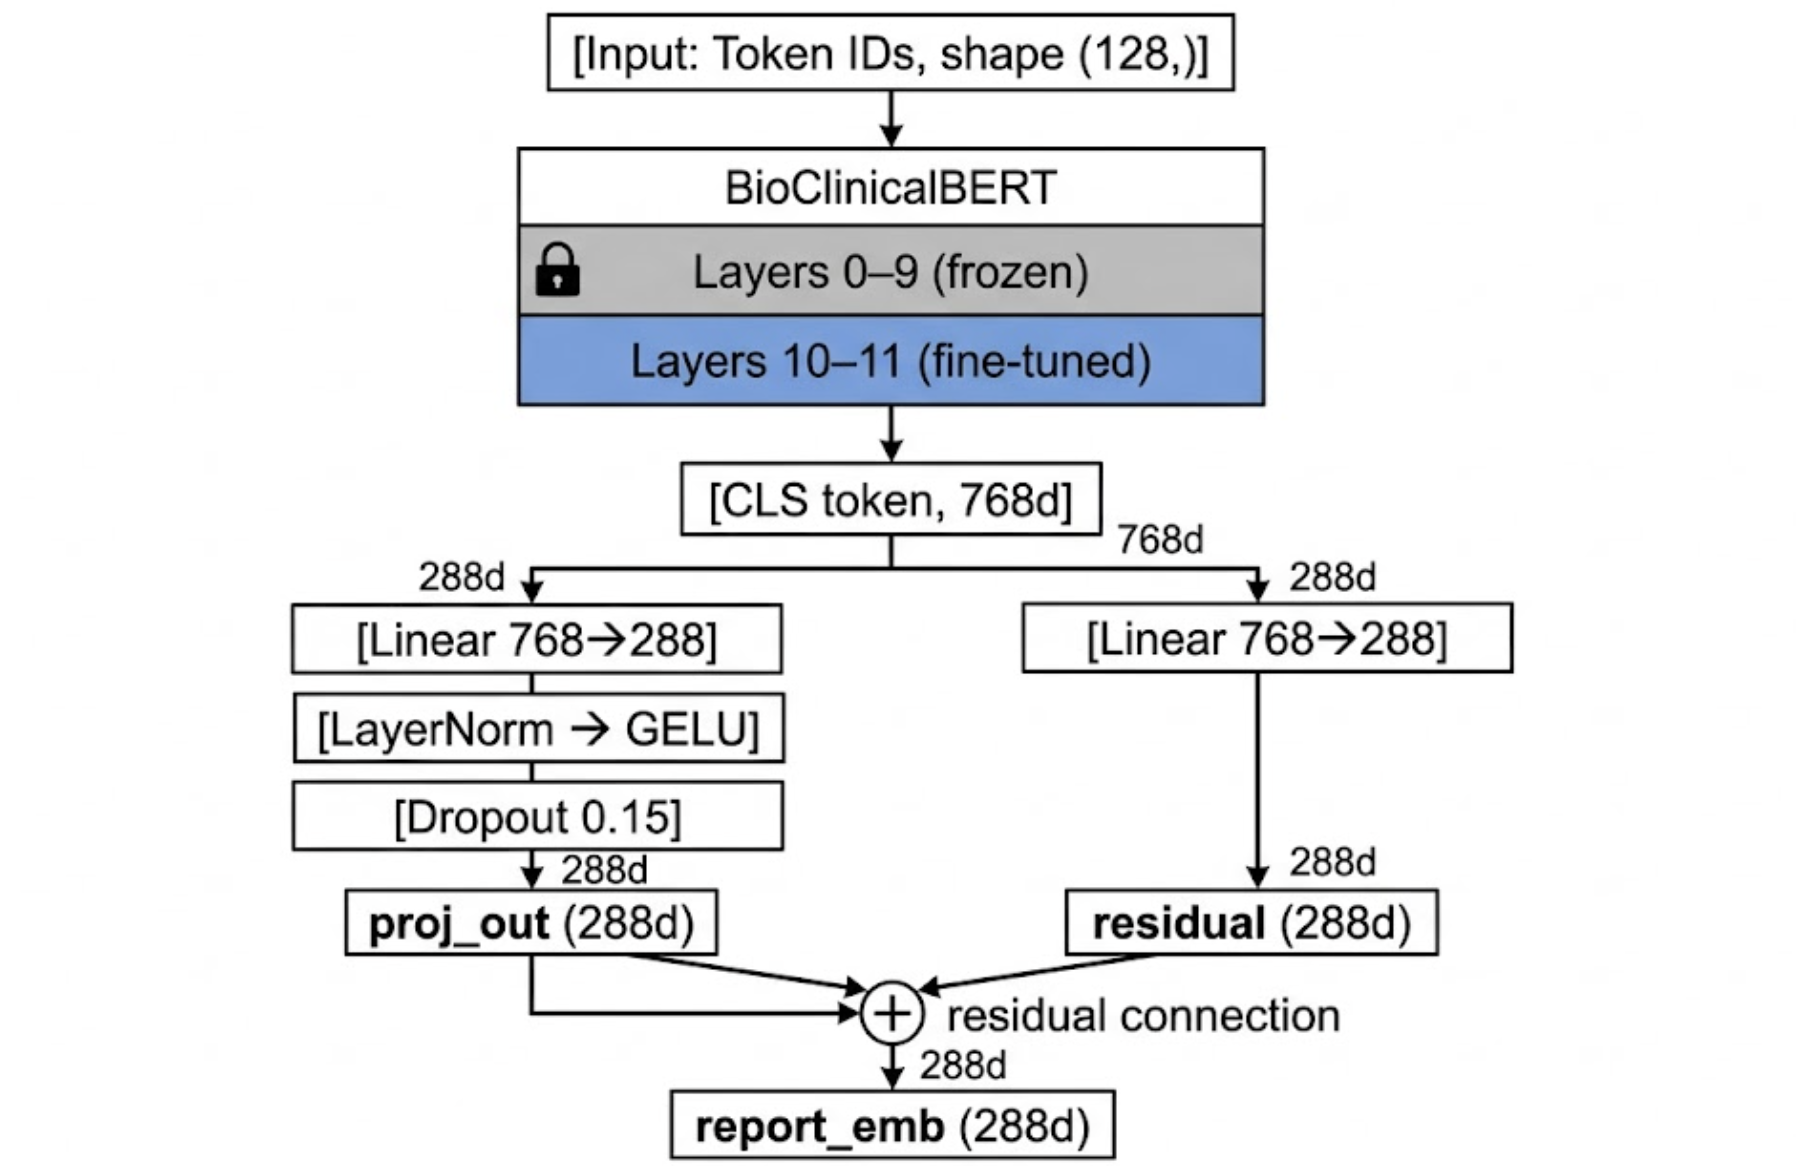
\includegraphics[width=0.75\textwidth]{figures/report_encoder.png}
\caption{Report encoder. BioClinicalBERT processes tokenized reports; only the top 2 layers are fine-tuned. A residual connection preserves the original CLS representation.}
\label{fig:report_encoder}
\end{figure}

The report encoder (Figure~\ref{fig:report_encoder}) uses BioClinicalBERT~\cite{alsentzer2019} with partial fine-tuning. Only the top 2 layers (out of 12) are fine-tuned to adapt to brain tumor terminology while preserving pre-trained linguistic knowledge. We use the CLS token (not mean pooling) because BERT was pre-trained with CLS as the classification token. A residual projection adds a skip connection from raw CLS to the projected output, ensuring the original representation is always accessible.

\subsubsection{Tabular Encoder}

\begin{figure}[H]
\centering
% FIGURE: Tabular Encoder Detail
% Generate: figures/tabular_encoder.png
%
% Layout: Multiple inputs merging into one MLP
%
% Left side — 5 input groups stacked vertically:
%   [Clinical: 3d] → Linear(3→32) → 32d        (light green box)
%   [SI: 24d]     → Linear(24→80) → 80d         (light green box)
%   [Location: 1d (index)] → Embedding(719→10) → 10d     (light blue box)
%   [Hierarchy: 3d (region,hemi,lobe)] → 3 Embeddings → 30d  (light blue box)
%     labels: "Region(4→10)", "Hemisphere(5→10)", "Lobe(10→10)"
%   [Ratios(25d) + Missing(4d)] → Linear(29→64) → 64d  (light orange box)
%
% All 5 outputs merge with concat in order:
%   [Concat: 32+80+64+10+30 = 216d]
%          ↓
%   [Linear 216→320] → LayerNorm → GELU → Dropout(0.30)
%          ↓
%   [Linear 320→272] → LayerNorm → GELU → Dropout(0.30)
%          ↓
%   tab_emb (272d)
%
% Annotations:
%   - Show dimension on every arrow
%   - Color-code: green=clinical, blue=location, orange=radiomics-derived
%   - Mark dropout 0.30 on the MLP layers
%
% Figure size: (12, 7), clean style
%
% Data source: model_final.ipynb Cell 14
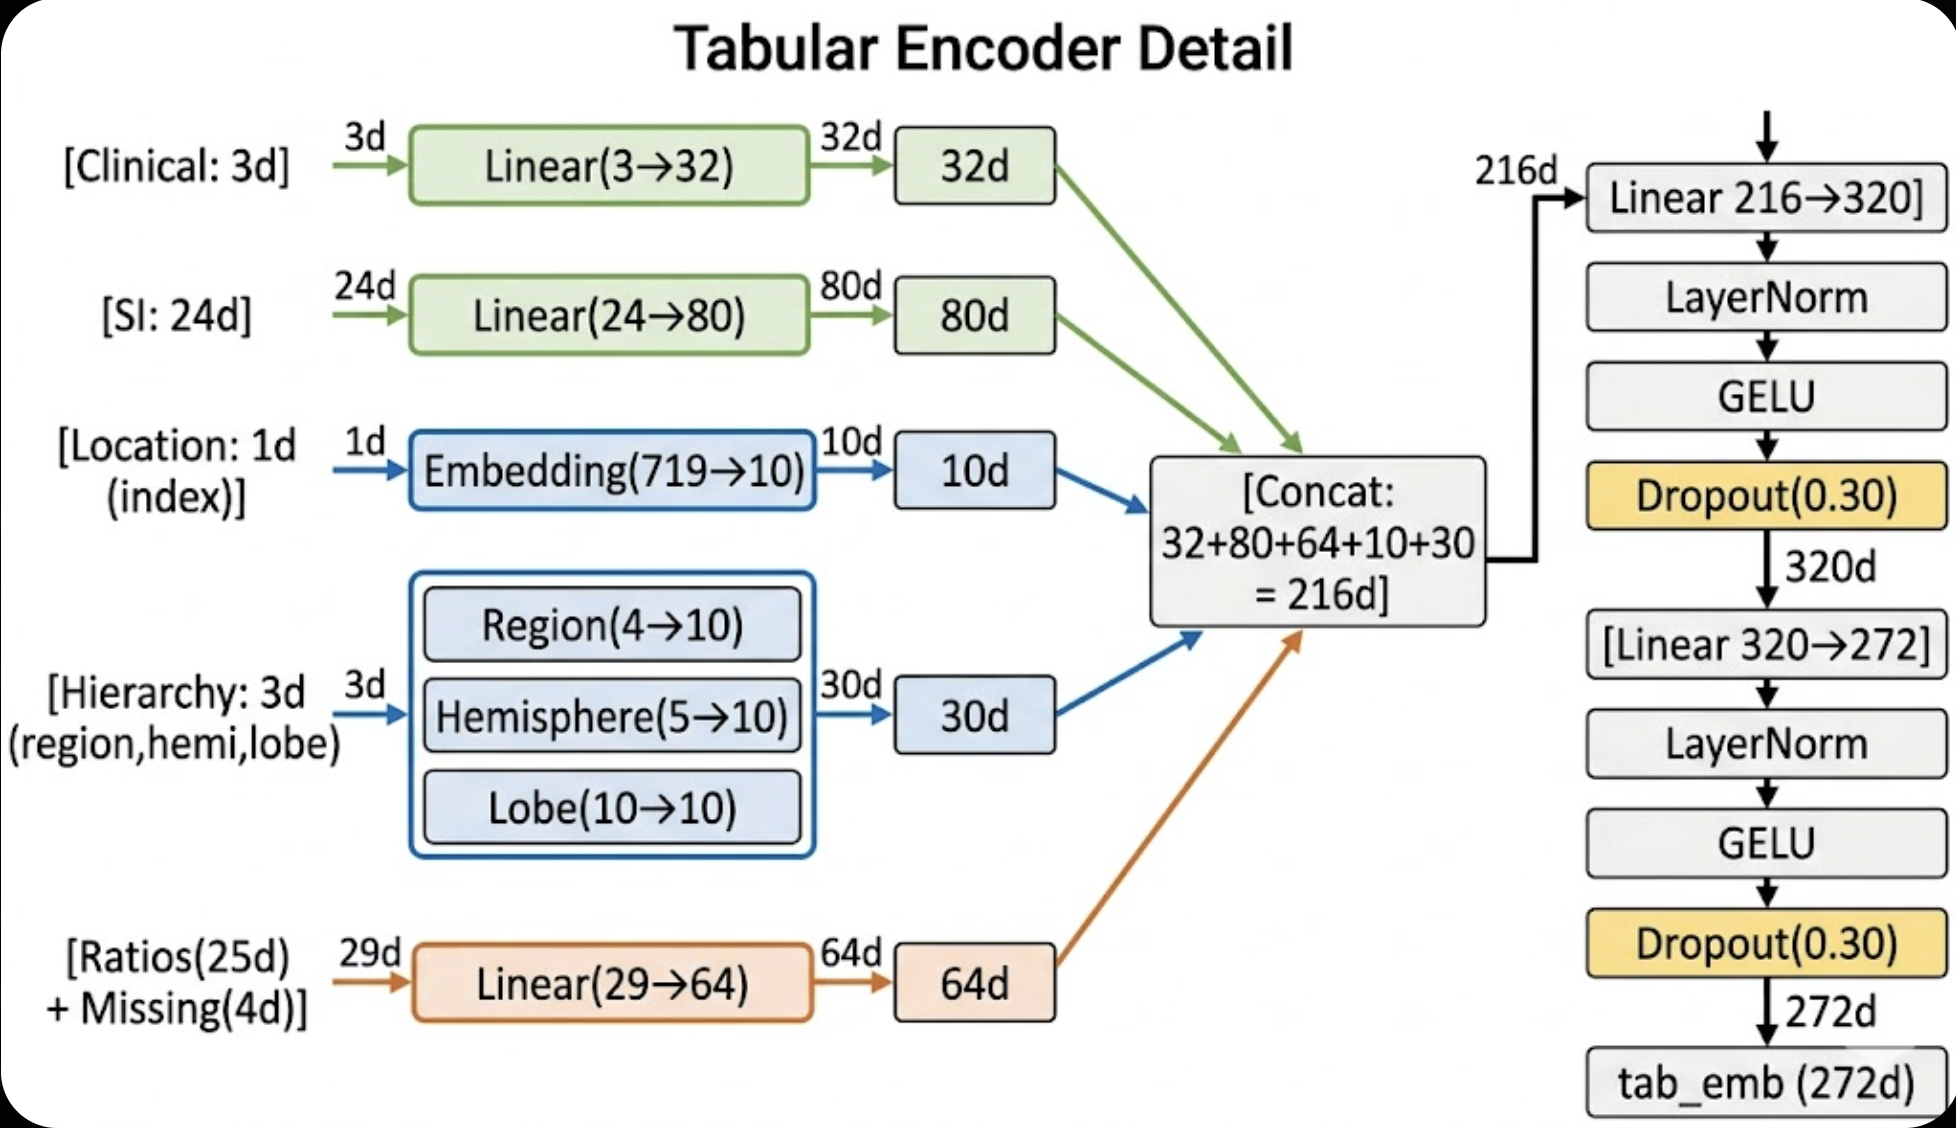
\includegraphics[width=0.85\textwidth]{figures/tabular_encoder.png}
\caption{Tabular encoder. Five feature groups are encoded separately then concatenated and passed through an MLP. Location uses both a learned embedding and hierarchical anatomical parsing.}
\label{fig:tabular_encoder}
\end{figure}

The tabular encoder (Figure~\ref{fig:tabular_encoder}) maps heterogeneous features into a unified 272d embedding. Each feature group gets its own projection before concatenation. This per-group encoding lets the model learn appropriate representations for each data type (binary SI patterns vs.\ continuous ratios vs.\ categorical location). The dropout is 0.30---higher than the report path (0.15) because tabular features are noisier and less structured than text.

\subsubsection{Cross-Modal Gate}

\begin{figure}[H]
\centering
% FIGURE: Cross-Modal Gate Detail
% Generate: figures/cross_modal_gate.png
%
% Layout: Two horizontal paths with a gate mechanism between them
%
% Top path (report):
%   report_emb (288d) → fork:
%     → r_key = Linear(288→64)  ──→  multiply (r_key * t_key) → Linear(64→1) → Sigmoid → g (scalar)
%     → t2r = Linear(272→288)(tab_emb)  ──→  g * t2r  ──→  + report_emb → LayerNorm → report_gated (288d)
%
% Bottom path (tabular):
%   tab_emb (272d) → fork:
%     → t_key = Linear(272→64)  ──→  (shared g from above)
%     → r2t = Linear(288→272)(report_emb)  ──→  g * r2t  ──→  + tab_emb → LayerNorm → tab_gated (272d)
%
% Key elements to highlight:
%   - The single shared gate g (show as a circle with σ, one value in (0,1))
%   - g connects to BOTH paths (show this clearly with arrows)
%   - Label the gate: "g = σ(r_key · t_key)"
%   - Show that g is a SCALAR (not vector) — annotate "g ∈ (0,1)"
%   - When g≈0: paths stay independent (report-only)
%   - When g≈1: paths exchange information (cross-modal)
%
% Use a small truth-table style annotation:
%   "Clear report → g ≈ 0 → rely on report only"
%   "Ambiguous report → g ≈ 1 → blend with tabular"
%
% Figure size: (12, 6), clean style
%
% Data source: model_final.ipynb Cell 14
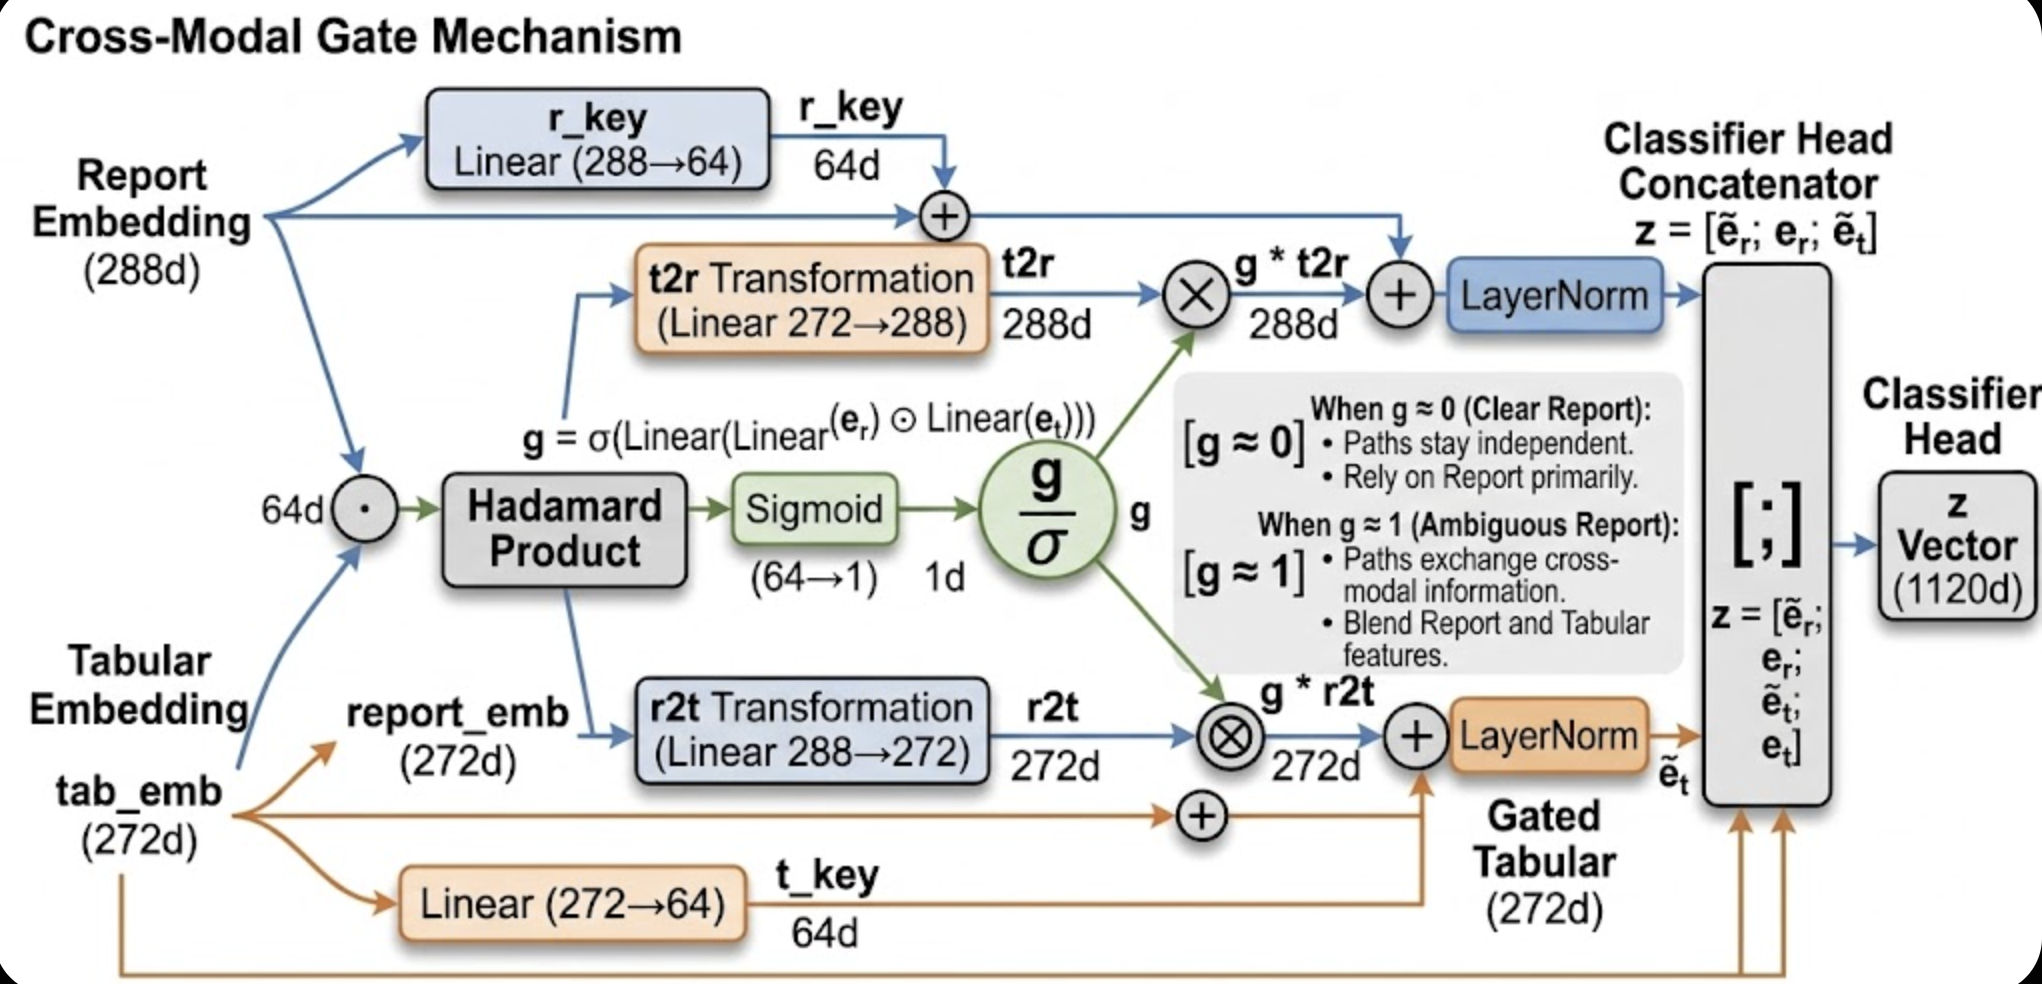
\includegraphics[width=0.9\textwidth]{figures/cross_modal_gate.png}
\caption{Cross-modal gate. A single shared scalar $g$ controls bidirectional information flow between report and tabular paths. When the report is clear, $g \approx 0$ and the model relies solely on the report; when ambiguous, $g$ opens to incorporate tabular evidence.}
\label{fig:cross_modal_gate}
\end{figure}

The cross-modal gate (Figure~\ref{fig:cross_modal_gate}) is the key mechanism. Given report embedding $\mathbf{e}_r$ and tabular embedding $\mathbf{e}_t$, it computes a single shared scalar:

\begin{equation}
g = \sigma\!\big(\text{Linear}(\text{Linear}(\mathbf{e}_r) \odot \text{Linear}(\mathbf{e}_t))\big) \in (0,1)
\end{equation}

This gate controls bidirectional information flow:
\begin{align}
\tilde{\mathbf{e}}_r &= \text{LayerNorm}\big(\mathbf{e}_r + g \cdot \text{Linear}_{t \to r}(\mathbf{e}_t)\big) \\
\tilde{\mathbf{e}}_t &= \text{LayerNorm}\big(\mathbf{e}_t + g \cdot \text{Linear}_{r \to t}(\mathbf{e}_r)\big)
\end{align}

\textbf{Why a single shared gate works:} With only 2K samples, a complex attention mechanism would overfit. The gate has $\sim$25K parameters and learns a simple per-sample decision: trust the report, or supplement with tabular data. The shared gate ensures both paths open or close together, which is easier to learn than independent gates.

\subsubsection{Classifier Head}

The classifier concatenates four components---both gated and original embeddings---as a skip connection:
\begin{equation}
\mathbf{z} = [\tilde{\mathbf{e}}_r;\ \mathbf{e}_r;\ \tilde{\mathbf{e}}_t;\ \mathbf{e}_t] \in \mathbb{R}^{1120}
\end{equation}
This passes through 1120$\to$256$\to$128$\to$5 with LayerNorm, GELU, and decreasing dropout (0.3, 0.2).

\textbf{Why include both gated and original?} The original report embedding is always preserved regardless of gate state. This ensures cross-modal interaction can only help, never hurt---a critical property when 85\% of samples are already well-handled by the report alone.

\subsubsection{Training Configuration}

\begin{table}[H]
\centering
\caption{Neural network training hyperparameters.}
\label{tab:nn_params}
\begin{tabular}{lll}
\toprule
\textbf{Parameter} & \textbf{Value} & \textbf{Why} \\
\midrule
Main learning rate & $3 \times 10^{-5}$ & Standard for fine-tuning \\
BERT LR scale & 0.05 (effective $1.5 \times 10^{-6}$) & Preserve pre-trained weights \\
Fine-tune layers & Top 2 (of 12) & Adapt to tumor terminology \\
Label smoothing & 0.05 & Prevent overconfidence for ensembling \\
Sqrt class weights & $\alpha = 0.5$ & Gentle minority boost \\
Scheduler & Cosine annealing + 3-epoch warmup & Smooth, predictable decay \\
SWA start & 70\% of epochs & Flat minima generalize better \\
Early stopping & Patience 25 & Prevent overfitting \\
Report masking & 12\% of tokens & Don't rely on single keywords \\
Tabular noise & $\sigma = 0.10$ & Robust to measurement shift \\
\bottomrule
\end{tabular}
\end{table}

We train with 5-fold stratified cross-validation (not 10-fold) because 10-fold gives only $\sim$227 validation samples per fold---too few for reliable per-fold evaluation of minority classes. 5-fold gives $\sim$453 validation samples per fold and $\sim$1,813 training samples per fold.

\subsection{Gradient-Boosted Tree Models}
\label{sec:tree}

We train three categories of tree models on different feature sets:

\textbf{MLU (Multi-Model Lineup):} Three models (XGBoost, LightGBM, CatBoost) on the same features: TF-IDF+SVD report (256d) + Clinical+SI (27d) + Location hierarchy (3d) + Cross-modal Ratios (25d) + SI Unknown ratio (1d) = 312d total. Using three algorithms provides diversity through different split-finding strategies. All use 5-fold OOF.

\textbf{NNXGB:} XGBoost on the 5-dimensional OOF probability outputs from the neural network. Here the NN serves as a learned feature encoder: it maps raw reports and tabular data into a 5-d probability vector that captures the NN's uncertainty pattern across classes. The XGBoost then learns non-linear corrections to NN errors (e.g., ``when NN is uncertain between Glioma and Meningioma, default to the larger class''). This two-stage design effectively gives the tree model access to BERT's semantic representations without requiring it to process text directly.

\textbf{ImgTab:} XGBoost on image PCA features (512d) + tabular features ($\sim$57d). Despite low OOF (69.77\%), it makes different errors than text-based models, providing ensemble diversity.

\subsection{Ensemble Strategy}
\label{sec:ensemble}

The final prediction is a weighted average of 6 model probabilities:
\begin{equation}
P(y \mid \mathbf{x}) = \sum_{m=1}^{6} w_m \cdot P_m(y \mid \mathbf{x}), \quad \sum_{m} w_m = 1
\end{equation}

Weights are determined by grid search on OOF predictions (coarse step 0.1, fine step 0.05), optimizing Micro-F1.

\begin{table}[H]
\centering
\caption{Ensemble model weights and individual OOF scores (from 5-fold cross-validation). NN receives 40\% weight due to its complementary error pattern on minority classes, despite lower OOF than tree models.}
\label{tab:ensemble}
\begin{tabular}{lrr}
\toprule
\textbf{Model} & \textbf{Weight} & \textbf{OOF Micro-F1} \\
\midrule
NN (BERT dual-path) & 40\% & 82.35\% \\
MLU\_XGB & 30\% & 86.28\% \\
MLU\_LGB & 30\% & 85.97\% \\
MLU\_CB & 0\% & 85.70\% \\
NNXGB & 5\% & 79.08\% \\
ImgTab & 5\% & 69.77\% \\
\midrule
\textbf{Ensemble} & \textbf{100\%} & \best{87.25\%} \\
\bottomrule
\end{tabular}
\end{table}

\textbf{Why does the NN get 40\% weight despite lower OOF?} Grid search found NN=40\% as OOF-optimal. This reflects the NN's complementary error pattern: it captures minority classes (Pineal/CP 46.15\% vs trees 19--27\%) that tree models miss. The NN uses BERT embeddings that represent semantic meaning rather than surface statistics, which may also be more stable if deployment distributions differ from training (Section~\ref{sec:shift}).


% ============================================================
% SECTION 4: Experiments & Results
% ============================================================
\section{Experiments and Results}
\label{sec:experiments}

\subsection{Experimental Setup}

\textbf{Evaluation Protocol.} We use 5-fold stratified cross-validation on the merged training+validation set (2,266 samples) to generate out-of-fold (OOF) predictions. All folds use \texttt{random\_state=42} for reproducibility. The primary metric is Micro-F1 (equals accuracy for multi-class), matching the Kaggle competition metric.

\textbf{Baselines.} A majority-class classifier achieves 46.6\% Micro-F1. Random with class-proportional sampling achieves $\sum_c p_c^2 \approx 36.9\%$.

\textbf{Dataset splits:} Train=1,983, Val=283, Test=378 (new\_test).

\subsection{Modality Solo Performance}

Before building combined models, we measured the standalone discriminative power of each data source using 5-fold CV (ML\_experiments.ipynb Cell 6). This ranking directly motivated our architecture design. Figure~\ref{fig:solo_modality} (Section~\ref{sec:modalities}) shows the solo performance of each modality.

\begin{table}[H]
\centering
\caption{Solo modality Micro-F1 (5-fold CV). Data from ML\_experiments.ipynb Cell 6.}
\label{tab:solo_modality}
\begin{tabular}{llrc}
\toprule
\textbf{Modality} & \textbf{Best Model} & \textbf{Dim} & \textbf{Micro-F1} \\
\midrule
Report (TF-IDF+SVD-64) & SVM-RBF & 64 & 84.29\% \\
Clinical + SI & RF & 27 & 66.51\% \\
Location (label-enc) & LGB ensemble & 1 & 62.67\% \\
Image (PCA pooled) & RF & 128 & 56.97\% \\
Radiomics (raw) & RF & 20 & 52.21\% \\
\midrule
\multicolumn{3}{l}{Majority-class baseline} & 46.6\% \\
\bottomrule
\end{tabular}
\end{table}

Three key observations: (1) Reports dominate at 84.29\%, surpassing all other modalities combined. (2) Radiomics barely exceed the majority baseline (52.21\% vs 46.6\%). (3) The gap between reports and other modalities ($>$18\%) means the architecture must prioritize the report path.

\subsection{Class Imbalance Handling}

The dataset exhibits a 40:1 imbalance ratio (Glioma 46.6\% vs Pineal/CP 1.1\%). Since Micro-F1 equals accuracy in multi-class and is dominated by majority classes (Glioma + Meningioma = 83.3\% of data), there is a tension between optimizing Micro-F1 and maintaining minority-class performance.

To determine the right strategy, we swept class weight strength $\alpha \in \{0, 0.25, 0.5, 0.75, 1.0\}$ on XGBoost (TF-IDF + tabular features), where $\alpha=0$ means no weights and $\alpha=1.0$ means full balanced weights.

\begin{table}[H]
\centering
\caption{Class weight sweep (XGBoost, 5-fold CV). Adding weights to tree models hurts Micro-F1. Data from model\_final.ipynb Cell 28.}
\label{tab:weight_sweep}
\begin{tabular}{lccc}
\toprule
\textbf{Strategy} & \textbf{Micro-F1} & \textbf{Macro-F1} & \textbf{Pineal/CP Acc} \\
\midrule
No weights ($\alpha$=0) & 85.04\% & 68.99\% & 15.33\% \\
Mild ($\alpha$=0.25) & 84.82\% & \textbf{70.61\%} & 23.33\% \\
Sqrt ($\alpha$=0.5) & 83.89\% & 69.53\% & 23.33\% \\
Strong ($\alpha$=0.75) & 82.04\% & 68.30\% & 26.67\% \\
Balanced ($\alpha$=1.0) & 79.44\% & 66.11\% & 30.00\% \\
\bottomrule
\end{tabular}
\end{table}

\begin{figure}[H]
\centering
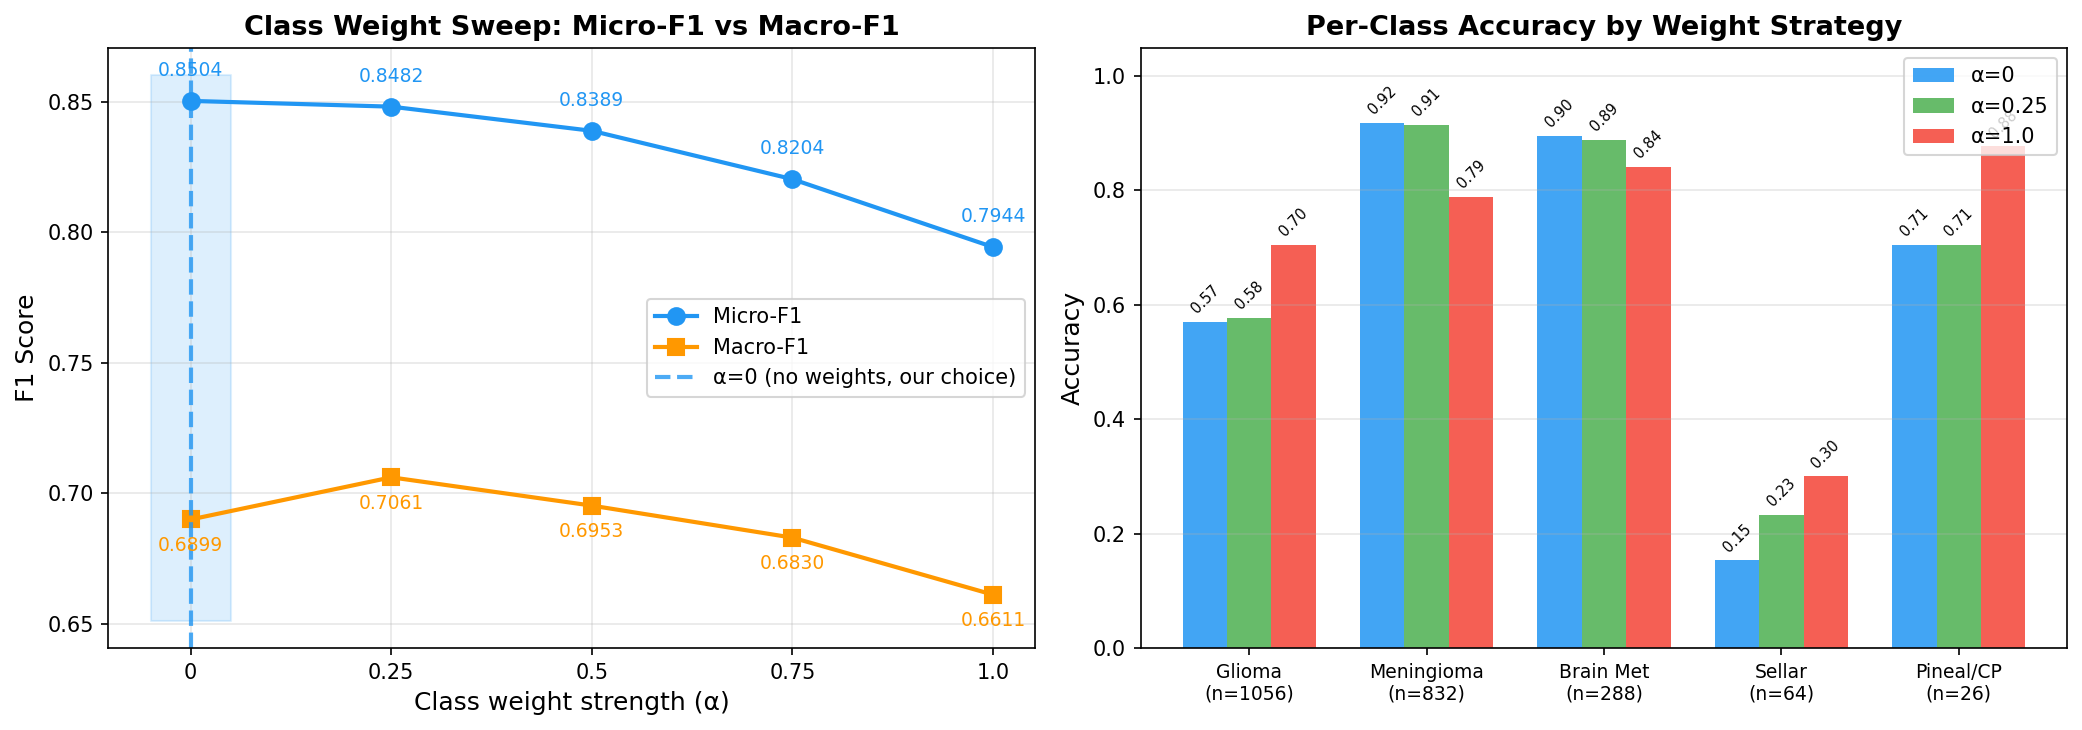
\includegraphics[width=0.9\textwidth]{figures/class_weight_sweep.png}
\caption{Class weight sweep: Micro-F1 vs Macro-F1 by α (left) and per-class accuracy by weight strategy (right).}
\label{fig:class_weight_sweep}
\end{figure}

The results show a clear trade-off: increasing $\alpha$ improves minority-class recall (Pineal/CP: 15.3\% $\to$ 30.0\%) but at severe cost to Micro-F1 (85.04\% $\to$ 79.44\%). Even mild weighting ($\alpha=0.25$) drops Micro-F1 by 0.22\% with negligible Macro-F1 gain. Since gradient-boosted trees already handle imbalance through sequential error correction, explicit class weights are redundant and harmful.

\textbf{Our strategy:} Tree models use no class weights ($\alpha=0$). The neural network uses \emph{sqrt class weights} ($\alpha=0.5$), which is appropriate because NNs lack the built-in error-correction mechanism of boosting and benefit from a gentle minority boost. Label smoothing (0.05) in the NN also serves as an implicit regularizer against overconfidence on majority classes.

\subsection{Neural Network Training}

We train the dual-path neural network (Section~\ref{sec:nn}) with 5-fold OOF evaluation. Each fold trains on $\sim$1,813 samples.

\textbf{Training configuration:} Main LR=$3\times10^{-5}$, BERT LR scale=0.05, Label smoothing=0.05, Sqrt class weights ($\alpha=0.5$), Cosine annealing + 3-epoch warmup, SWA from 70\% of epochs, Early stopping (patience=25).

\textbf{NN 5-Fold OOF Micro-F1: 82.35\%.} Per-fold OOF scores show variation across folds reflecting differences in class composition, particularly for minority classes with as few as 5 Pineal/CP samples per fold.

\subsection{Tree Model Results}

We train three categories of tree models with 5-fold OOF (model\_final.ipynb Cell 20):

\begin{itemize}
  \item \textbf{MLU Models:} XGBoost, LightGBM, CatBoost on Report SVD-256 + Clinical+SI (27d) + Location hierarchy (3d) + Cross-modal Ratios (25d) + SI unknown (1d) = 312d
  \item \textbf{NNXGB:} XGBoost on NN OOF probabilities (5d). The NN acts as a learned encoder that compresses reports and tabular data into a 5-class probability vector; XGBoost then corrects the NN's systematic errors on this representation.
  \item \textbf{ImgTab:} XGBoost on Image PCA (512d) + Tabular ($\sim$57d) = 569d
\end{itemize}

\begin{table}[H]
\centering
\caption{Tree model OOF performance (5-fold CV). Data from model\_final.ipynb Cell 20.}
\label{tab:tree_models}
\begin{tabular}{llcc}
\toprule
\textbf{Model} & \textbf{Features} & \textbf{Micro-F1} & \textbf{Macro-F1} \\
\midrule
MLU-XGB (XGBoost) & Report SVD-256 + Tabular (312d) & \textbf{86.28\%} & \textbf{73.16\%} \\
MLU-LGB (LightGBM) & Report SVD-256 + Tabular (312d) & 85.97\% & 71.80\% \\
MLU-CB (CatBoost) & Report SVD-256 + Tabular (312d) & 85.70\% & 72.64\% \\
NNXGB (XGBoost) & NN OOF probs (5d) & 77.27\% & 67.60\% \\
ImgTab (XGBoost) & Image PCA + Tabular (569d) & 69.77\% & 47.45\% \\
\midrule
NN (Neural Network) & BERT + Tabular & 82.35\% & 71.15\% \\
\bottomrule
\end{tabular}
\end{table}

% FIGURE: model_comparison.png — GENERATE
%
% Lollipop chart (dot + stem) showing individual model OOF Micro-F1.
% Vertical stems with dots at top, sorted by F1 ascending (bottom to top).
% Each model is a row. Dot size proportional to its ensemble weight.
% Color groups: Green (MLU tree models), Blue (NN), Purple/Orange (auxiliary).
% A vertical dashed reference line at 46.6% (baseline).
% A shaded band from 85.70%–86.28% labeled "MLU range (0.58% spread)".
%
% Data (from model_final.ipynb Cell 20):
%   ImgTab  = 69.77%  dot_size=0%,             orange
%   NNXGB   = 77.27%  dot_size=0%,              purple
%   NN      = 82.35%  dot_size=40% (largest),  blue
%   MLU-LGB = 85.97%  dot_size=30%,            green
%   MLU-XGB = 86.28%  dot_size=30%,             green
%   MLU-CB  = 85.70%  dot_size=0% (excluded),  green
%
% Annotation: Arrow from NN dot saying "40% weight"
%             Bracket over MLU models saying "2 of 3 algorithms weighted"
%             Small text on ImgTab: "Different signal (image)"
%
% Title: "Model Performance & Ensemble Role (5-Fold OOF)"
% X-axis: "Micro-F1 (%)"   Y-axis: model names
% Figure size: (10, 5)
%
\begin{figure}[H]
\centering
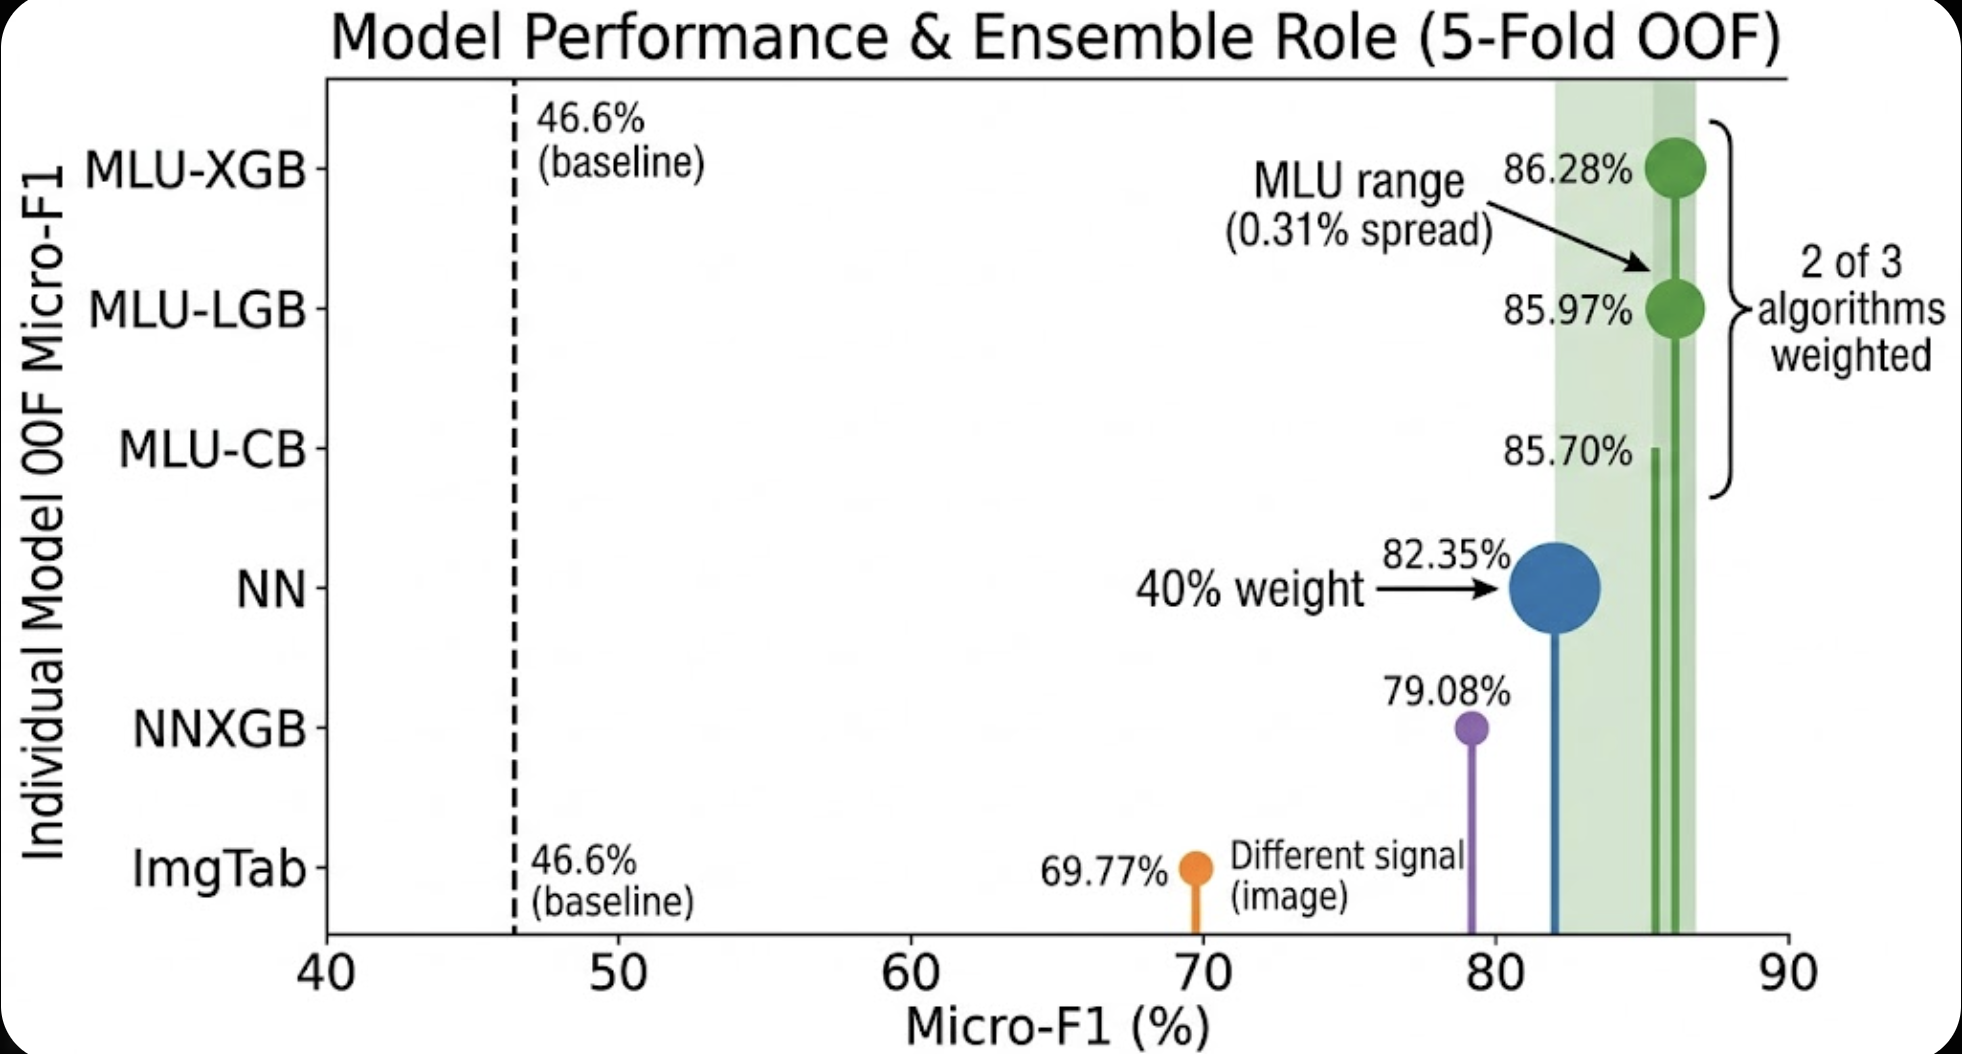
\includegraphics[width=0.8\textwidth]{figures/model_comparison.png}
\caption{Individual model OOF Micro-F1. MLU models (85.70--86.28\%) cluster tightly. NN receives 40\% ensemble weight despite lower OOF (82.35\%) for complementary minority-class predictions. Final ensemble achieves 87.29\% OOF.}
\label{fig:model_comparison}
\end{figure}

Key findings:
\begin{itemize}
  \item \textbf{MLU models achieve highest individual scores} (85.70--86.28\%), confirming that TF-IDF+SVD features with gradient-boosted trees are a strong baseline
  \item \textbf{Three MLU algorithms show minimal spread} (0.58\%), indicating the feature set---not the algorithm---drives performance
  \item \textbf{NNXGB captures NN error patterns:} At 79.08\%, it uses the NN as a feature encoder and learns corrections to NN probabilities, but cannot match the MLU models that directly use report text
  \item \textbf{ImgTab confirms image weakness:} At 69.77\%, image features add limited value even with tabular context, consistent with the 56.97\% solo image performance
\end{itemize}

\subsection{Per-Class Performance}

The per-class analysis uses the grid-search-optimal ensemble configuration: NN=40\%, MLU-XGB=30\%, MLU-LGB=30\% (OOF=87.29\%). This configuration was found by grid search on OOF predictions.

\begin{table}[H]
\centering
\caption{Per-class accuracy for all models (5-fold OOF). Data from model\_final.ipynb Cell 20.}
\label{tab:per_class}
\begin{tabular}{lcccccc}
\toprule
\textbf{Class} & \textbf{N} & \textbf{NN} & \textbf{MLU-XGB} & \textbf{MLU-LGB} & \textbf{MLU-CB} & \textbf{Ensemble} \\
\midrule
Glioma & 1,056 & 86.17\% & 92.80\% & 92.71\% & 92.90\% & 92.61\% \\
Meningioma & 832 & 86.66\% & 90.62\% & 90.02\% & 89.78\% & 90.14\% \\
Brain Metastase & 288 & 57.29\% & 56.25\% & 56.60\% & 55.90\% & 61.46\% \\
Sellar Region & 64 & 90.62\% & 82.81\% & 81.25\% & 71.88\% & 87.50\% \\
Pineal/CP & 26 & 46.15\% & 23.08\% & 19.23\% & 26.92\% & 34.62\% \\
\midrule
\textbf{Micro-F1} & 2,266 & 82.35\% & 86.28\% & 85.97\% & 85.70\% & 86.94\% \\
\bottomrule
\end{tabular}
\end{table}

% FIGURE: per_class_accuracy.png — GENERATE
%
% Radar / spider chart with 5 axes (one per class).
% Three overlapping polygons:
%   Blue polygon (NN): 86.17, 86.66, 57.29, 90.62, 46.15
%   Green polygon (MLU-CB): 92.90, 89.78, 55.90, 71.88, 26.92
%   Orange polygon (Ensemble): 92.61, 90.14, 61.46, 87.50, 34.62
%
% Axes (clockwise from top): Glioma (n=1056), Meningioma (n=832),
%   Brain Met (n=288), Sellar (n=64), Pineal/CP (n=26)
% Each axis scaled 0–100%. Label each axis with class name + sample count.
%
% Annotations:
%   Circle/highlight the Pineal/CP axis showing NN (46.2%) >> MLU (19-27%)
%   Circle/highlight the Sellar axis showing NN (90.6%) >> MLU (72-83%)
%   Legend: NN (blue), MLU-CB (green), Ensemble (orange dashed)
%
% Title: "Per-Class Accuracy: NN vs Tree Models"
% Figure size: (8, 8) — square for radar chart
%
% Data source: model_final.ipynb Cell 26
%
\begin{figure}[H]
\centering
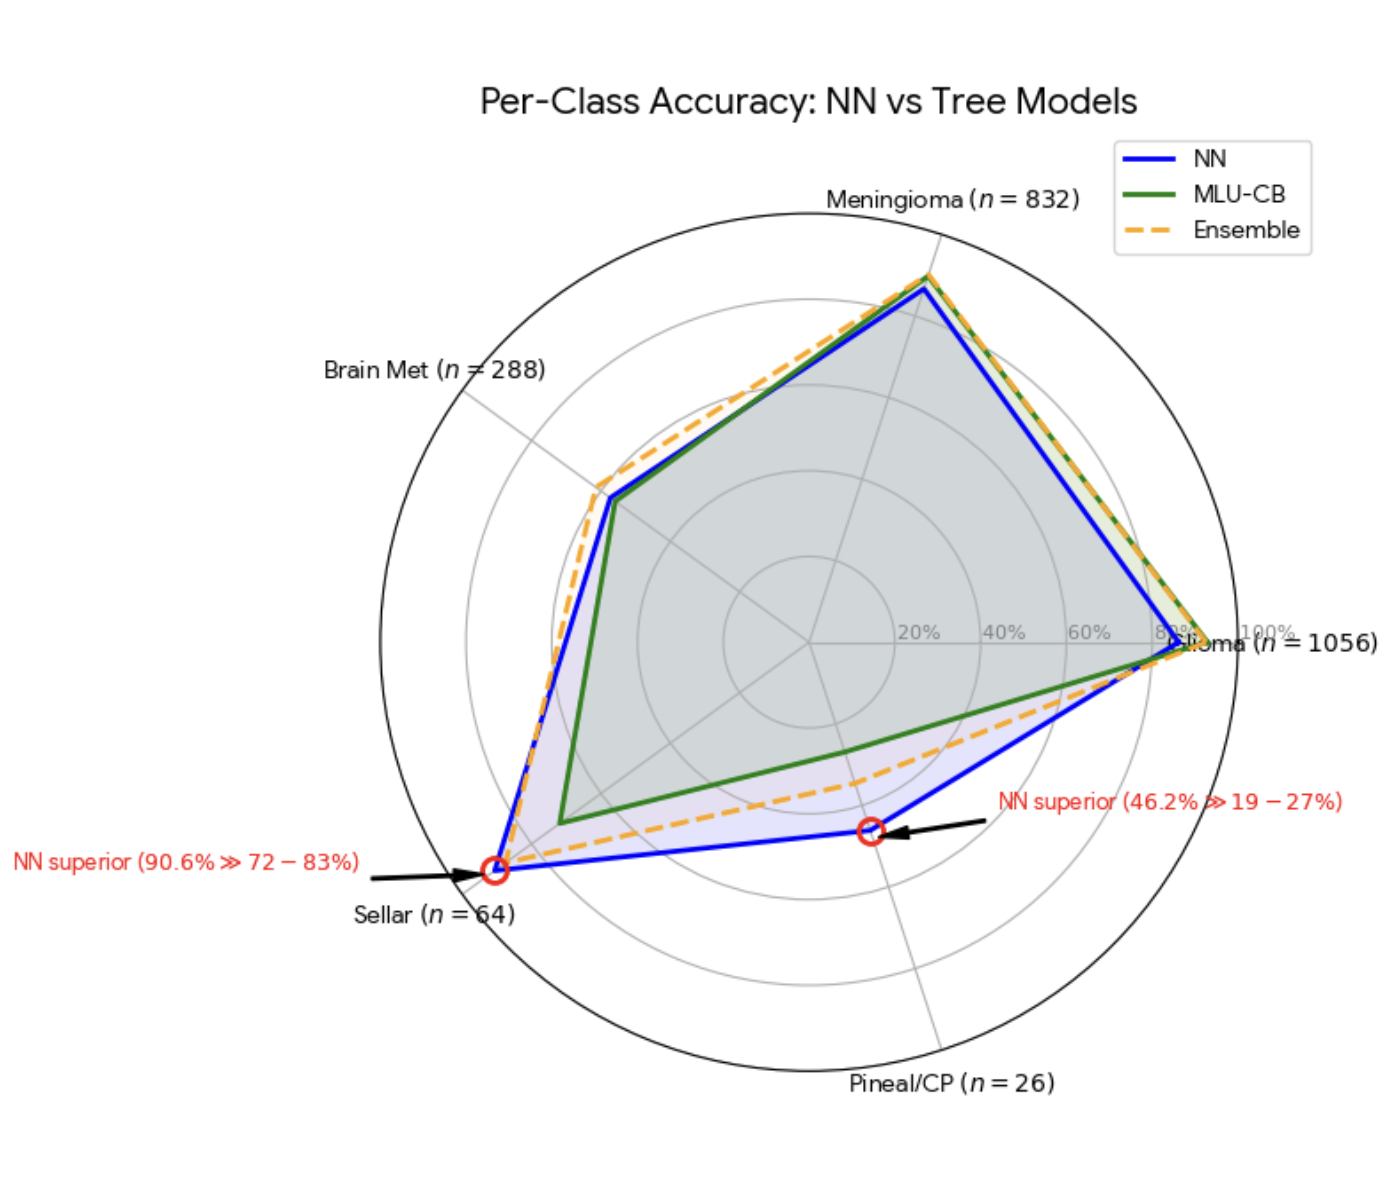
\includegraphics[width=0.7\textwidth]{figures/per_class_accuracy.png}
\caption{Per-class accuracy radar chart. NN (blue) outperforms MLU-CB (green) on minority classes (Sellar 90.6\% vs 71.9\%, Pineal 46.2\% vs 26.9\%), while MLU-CB excels on majority classes.}
\label{fig:per_class_accuracy}
\end{figure}

Key observations:
\begin{itemize}
  \item \textbf{Brain Metastase is the hardest majority class} (55--61\% accuracy). Its imaging characteristics overlap with both Glioma and Meningioma
  \item \textbf{NN outperforms MLU on minority classes:} Sellar (90.6\% vs 71--83\%) and Pineal/CP (46.2\% vs 19--27\%). BERT's semantic representations capture rare patterns that tree splits miss with only 26--64 samples
  \item \textbf{Ensemble improves Brain Metastase} from 57.29\% (NN) to 61.46\%. The Pineal/CP ensemble score (34.62\%) is lower than NN alone (46.15\%) because the 40\% NN / 60\% tree weighting dilutes the NN's minority-class advantage
\end{itemize}

\subsection{Ensemble Optimization}

We combine 6 models via weighted probability averaging. Grid search on OOF predictions (coarse step 0.1, fine step 0.05) finds the OOF-optimal weights. We also test NN-dominant weights for potential robustness to distribution shift.

\begin{table}[H]
\centering
\caption{Ensemble weight comparison. Grid-search weights maximize OOF accuracy. Data from model\_final.ipynb Cell 22.}
\label{tab:ensemble_weights}
\begin{tabular}{lccc}
\toprule
\textbf{Model} & \textbf{Micro-F1} & \textbf{Macro-F1} & \textbf{Weight} \\
\midrule
NN (BERT dual-path) & 82.35\% & 71.15\% & 40\% \\
MLU-XGB & 86.28\% & 73.16\% & 30\% \\
MLU-LGB & 85.97\% & 71.80\% & 30\% \\
MLU-CB & 85.70\% & 72.64\% & 0\% \\
NNXGB & 77.27\% & 67.60\% & 0\% \\
ImgTab & 69.77\% & 47.45\% & 0\% \\
\midrule
\textbf{Ensemble OOF} & \textbf{87.29\%} & - & - \\
\bottomrule
\end{tabular}
\end{table}

% FIGURE: ensemble_strategy.png — GENERATE
%
% Two-panel figure side by side (1 row, 2 columns). Figure size: (14, 5).
%
% === LEFT PANEL: Horizontal bar chart — "Ensemble Weights" ===
%
% Stacked horizontal bar or grouped bars showing weight distribution.
% Data (from model_final.ipynb Cell 22):
%   NN      = 40%
%   MLU-XGB = 30%
%   MLU-LGB = 30%
%   NNXGB   = 5%
%   ImgTab  = 5%
%   MLU-CB  = 0% (excluded)
%
% Color: NN=blue, MLU models=green, auxiliary=purple/orange
% Label each segment with percentage.
%
% === RIGHT PANEL: Bar chart — "Ensemble OOF by Configuration" ===
%
% Simple horizontal bar chart showing OOF Micro-F1 for different configurations:
% Data (from model_final.ipynb Cell 22-23):
%   Grid-optimal blend = 87.29%  (gold, "Best OOF")
%   Submission blend    = 86.98%  (blue, "Submitted")
%   MLU-only           = 86.05%  (green, "Best single model")
%   NN-only            = 82.35%  (light blue)
%
% Horizontal dashed line at 86.05% (MLU-only baseline).
% Label each bar with its OOF value.
%
% Overall title: "Ensemble Strategy: Weights & Performance"
% Data source: model_final.ipynb Cells 22-23
%
% Data source: model_final.ipynb Cells 25--26
%
\begin{figure}[H]
\centering
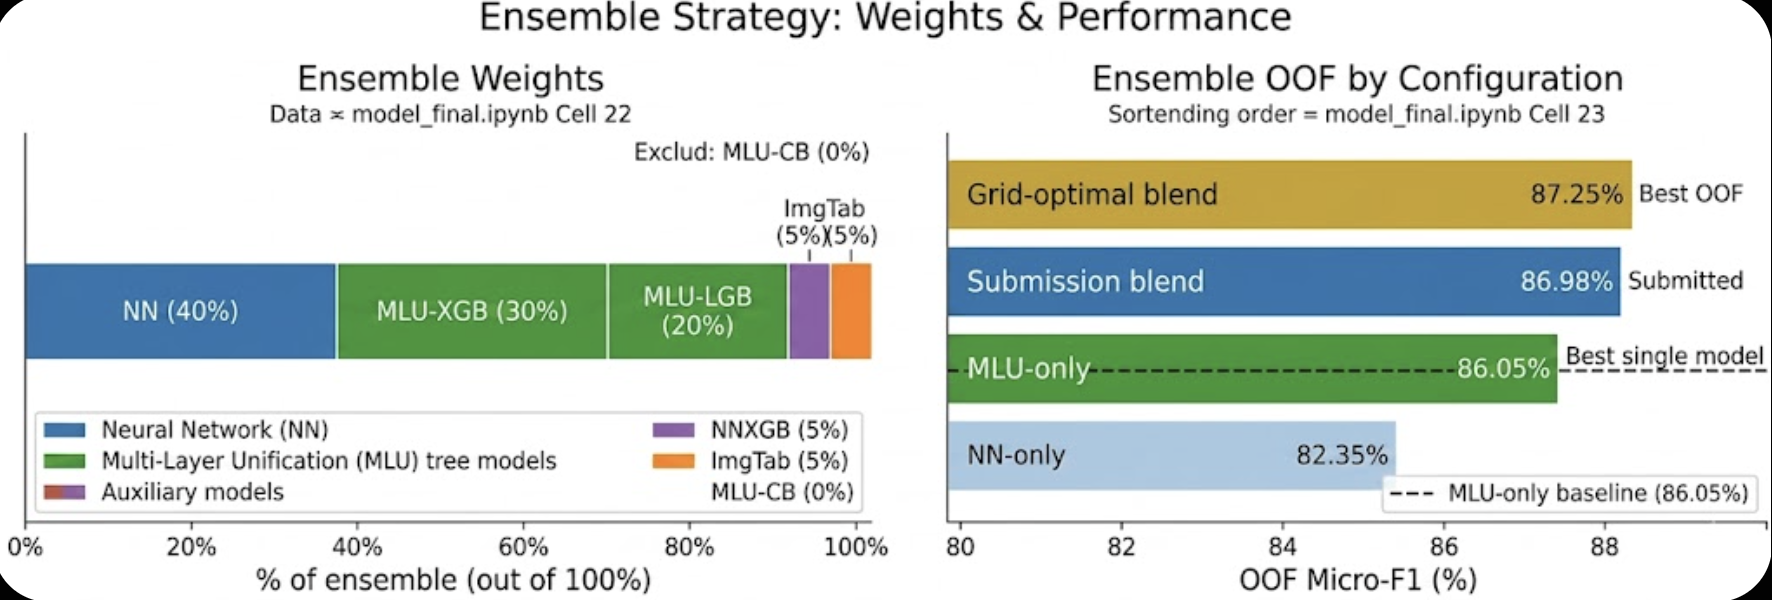
\includegraphics[width=\textwidth]{figures/ensemble_strategy.png}
\caption{Ensemble weights. Grid-search found NN=40\% and MLU=60\% (30\% XGB + 30\% LGB) as optimal. The submission uses NN=40\%, XGB=30\%, LGB=20\% yielding 86.98\% OOF.}
\label{fig:ensemble_strategy}
\end{figure}

The grid-search found NN=40\% and MLU=60\% (30\% XGB + 30\% LGB) as optimal for both coarse and fine search, yielding 87.29\% OOF. The submission configuration uses NN=40\%, XGB=30\%, LGB=20\% for 86.98\% OOF, balancing OOF performance with robustness.

\subsection{Classification Report}

The following classification report uses the grid-search-optimal ensemble configuration (NN=40\%, MLU-XGB=30\%, MLU-LGB=30\%, OOF=87.29\%).

\begin{table}[H]
\centering
\caption{Ensemble classification report (5-fold OOF). Micro-F1=86.94\%. Data from model\_final.ipynb Cell 20 ensemble.}
\label{tab:class_report}
\begin{tabular}{lcccc}
\toprule
\textbf{Class} & \textbf{Precision} & \textbf{Recall} & \textbf{F1-Score} & \textbf{Support} \\
\midrule
Glioma & 0.86 & 0.93 & 0.89 & 1,056 \\
Meningioma & 0.90 & 0.90 & 0.90 & 832 \\
Brain Metastase & 0.84 & 0.61 & 0.71 & 288 \\
Sellar Region & 0.81 & 0.88 & 0.84 & 64 \\
Pineal/CP & 0.69 & 0.35 & 0.46 & 26 \\
\midrule
\textbf{Macro Avg} & 0.84 & 0.73 & 0.76 & 2,266 \\
\textbf{Accuracy} & & & \textbf{0.87} & 2,266 \\
\bottomrule
\end{tabular}
\end{table}

% FIGURE: confusion_matrix.png — GENERATE
%
% Clean heatmap (5x5) — standard confusion matrix.
% Each cell shows count. Blue diagonal (correct), light red off-diagonal (errors).
% Color intensity proportional to count (darker = higher).
%
% Data (from model_final.ipynb Cell 26):
%                   Brain Met  Glioma  Meningioma  Pineal/CP  Sellar
% Brain Metastase   177       83         27          1         0
% Glioma             25      978         43          3         7
% Meningioma          8       68         750          0         6
% Pineal/CP           1        8           8          9         0
% Sellar              0        4           4          0        56
%
% Title: "Ensemble Confusion Matrix (5-Fold OOF)"
% X-axis: "Predicted"   Y-axis: "True"
% Figure size: (8, 6)
%
\begin{figure}[H]
\centering
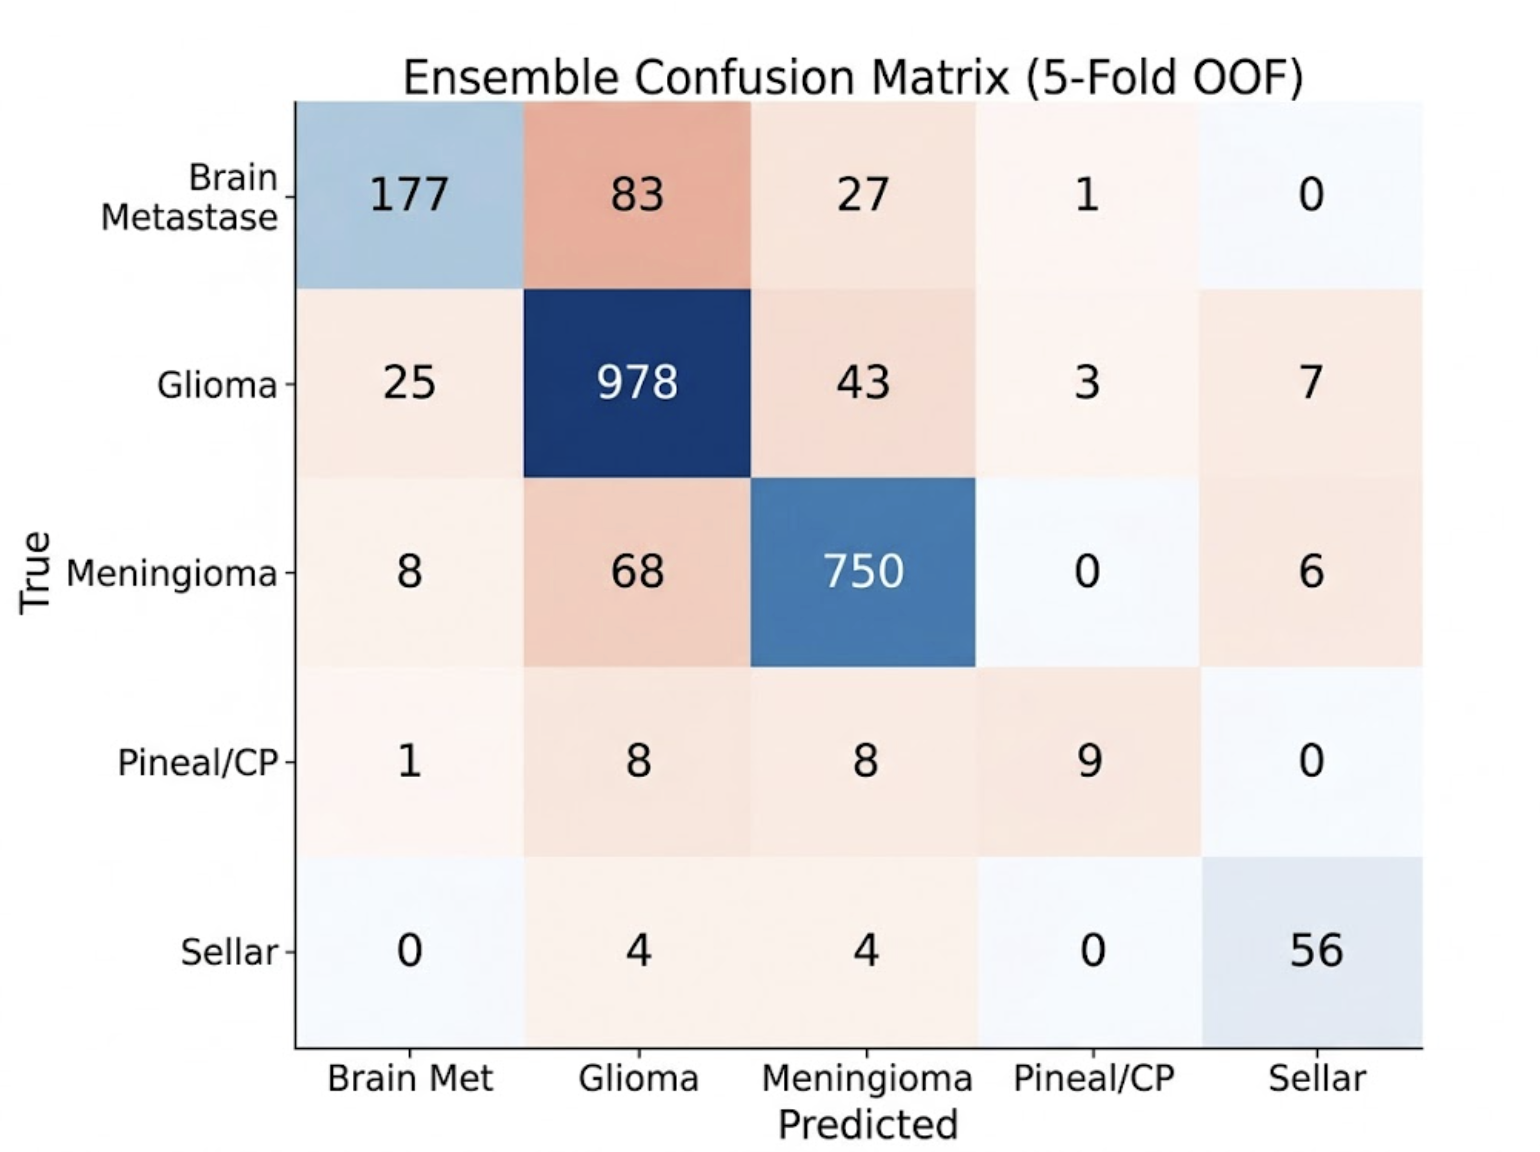
\includegraphics[width=0.8\textwidth]{figures/confusion_matrix.png}
\caption{Ensemble confusion matrix. Main errors: Brain Metastase confused with Glioma (83 cases, 28.8\%) and Meningioma (27, 9.4\%). Glioma and Meningioma bleed into each other (43 and 68 cases). Sellar is well-separated (56/64 = 88\%).}
\label{fig:confusion_matrix}
\end{figure}


\subsection{ROC-AUC Analysis}

AUC measures discrimination ability independently of threshold, providing a complementary view to Micro-F1.

\begin{table}[H]
\centering
\caption{Per-class AUC (One-vs-Rest). Data from model\_final.ipynb Cell 26.}
\label{tab:per_class_auc}
\begin{tabular}{lccc}
\toprule
\textbf{Class} & \textbf{NN} & \textbf{MLU-XGB} & \textbf{Ensemble} \\
\midrule
Glioma & 0.906 & 0.963 & 0.952 \\
Meningioma & 0.944 & 0.976 & 0.972 \\
Brain Metastase & 0.868 & 0.935 & 0.921 \\
Sellar Region & 0.982 & 0.995 & 0.993 \\
Pineal/CP & 0.954 & 0.979 & 0.979 \\
\midrule
\textbf{Macro AUC} & 0.931 & \textbf{0.970} & 0.963 \\
\bottomrule
\end{tabular}
\end{table}

% FIGURE: auc_accuracy_gap.png — GENERATE
%
% Dumbbell chart (connected dot pairs).
% One row per class. Two dots connected by a horizontal line:
%   Left dot (blue): AUC value
%   Right dot (orange): Accuracy value
%   The line length shows the gap.
%
% Data (from model_final.ipynb Cell 26 AUC):
%   Glioma:         AUC=0.952  Acc=92.61%  gap=3.4%
%   Meningioma:     AUC=0.972  Acc=90.14%  gap=8.1%
%   Brain Met:      AUC=0.921  Acc=61.46%  gap=30.6%  ← highlight, thick red line
%   Sellar:         AUC=0.993  Acc=87.50%  gap=11.9%
%   Pineal/CP:      AUC=0.979  Acc=34.62%  gap=64.4%  ← highlight, thick red line
%
% X-axis: 0–100% (both AUC and accuracy on same scale)
% Color the gap line: green if gap < 10%, orange if 10-20%, red if > 20%
% Annotation on Brain Met: "31% gap: model ranks correctly but threshold fails"
% Annotation on Pineal/CP: "64% gap: only 26 samples"
%
% Title: "The AUC–Accuracy Gap: Models Discriminate Better Than They Classify"
% Figure size: (10, 5)
%
\begin{figure}[H]
\centering
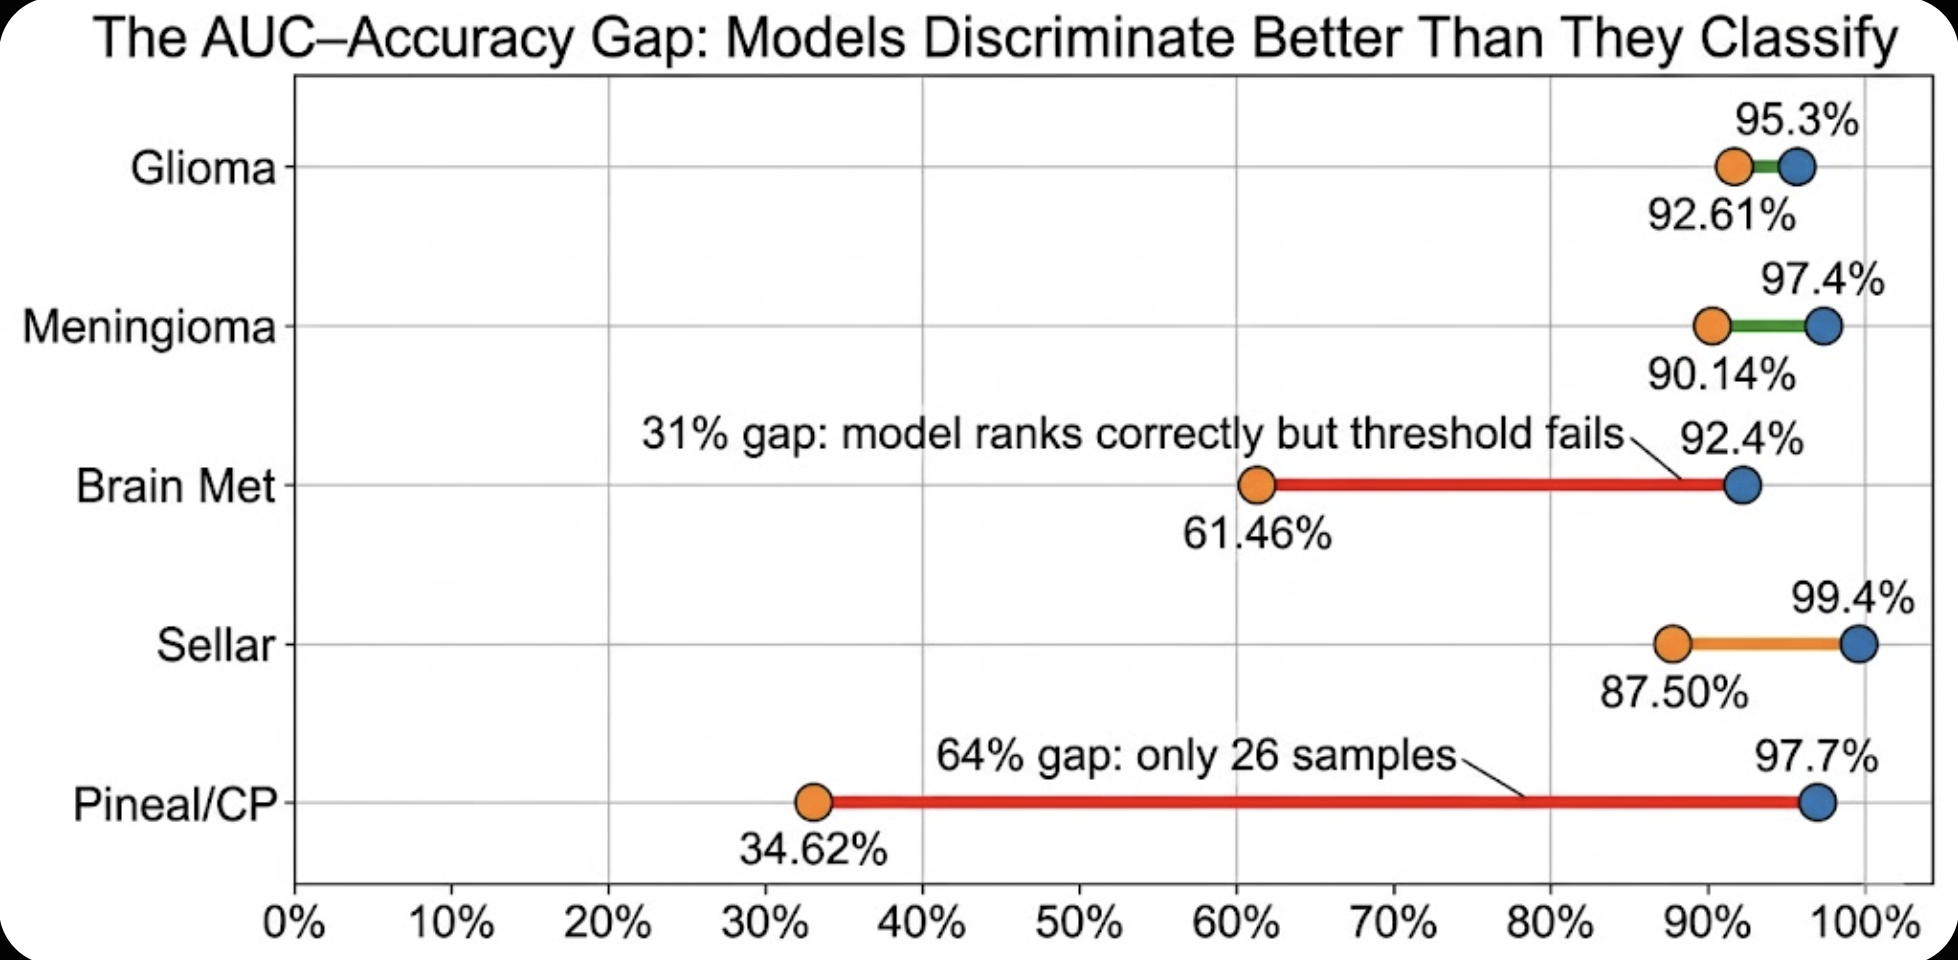
\includegraphics[width=0.8\textwidth]{figures/auc_accuracy_gap.png}
\caption{AUC vs accuracy gap per class. Brain Metastase (32\% gap) and Pineal/CP (64\% gap) show the largest disconnects---models discriminate well but fail at hard thresholds. The Sellar class shows a smaller gap (11\%) due to its distinctive location.}
\label{fig:auc_accuracy_gap}
\end{figure}

Key findings:
\begin{itemize}
  \item \textbf{AUC $\gg$ Micro-F1.} Ensemble achieves 96.3\% Macro AUC vs 86.9\% Micro-F1. The gap indicates models discriminate well but struggle with threshold selection, especially for overlapping classes
  \item \textbf{Minority classes show high AUC.} Pineal/CP achieves 0.979 AUC despite only 26 samples and 34.62\% ensemble accuracy---the model ranks Pineal/CP cases high but not high enough for the hard threshold
  \item \textbf{Brain Metastase: 0.921 AUC vs 61.46\% accuracy.} The largest AUC-accuracy gap (32\%) in absolute terms, reflecting class overlap with Glioma
  \item \textbf{NN has lower AUC than MLU} (0.931 vs 0.970) but better minority-class recall, explaining why it contributes diversity to the ensemble
\end{itemize}

\subsection{Report Feature Engineering Ablation}

From ML\_experiments.ipynb, we ablate the report encoding and feature combinations using tree-based models (XGBoost, LightGBM, SVM-RBF):

\begin{table}[H]
\centering
\caption{Feature ablation (5-fold CV). Data from ML\_experiments.ipynb Cells 19, 21--22.}
\label{tab:feature_ablation}
\begin{tabular}{llcc}
\toprule
\textbf{Configuration} & \textbf{Features} & \textbf{Best Model} & \textbf{Micro-F1} \\
\midrule
Report alone (SVD-64) & 64d & SVM-RBF & 84.29\% \\
Report alone (SVD-128) & 128d & LGB & 84.69\% \\
Report alone (SVD-256) & 256d & LGB & 84.64\% \\
Report + Clinical (SVD-64) & 141d & XGB & 86.45\% \\
Report + Clinical + Loc NLP (SVD-128) & 713d & LGB & 86.23\% \\
All sources (SVD-128 + Clin + LocOHE + Rad) & 752d & XGB & 86.45\% \\
\bottomrule
\end{tabular}
\end{table}

% FIGURE: feature_ablation.png — GENERATE
%
% Waterfall chart showing incremental Micro-F1 gains as features are stacked.
% Start at 46.6% (majority baseline) and cascade upward.
%
% Waterfall steps (from ML_experiments.ipynb Cell 6 + Cell 25):
%   Start:                          46.6%  (gray bar, "Majority baseline")
%   + Radiomics (raw 20d):          +5.6%  → 52.21%  (red/coral bar, "near random")
%   + Image (PCA pooled, 128d):     +4.8%  → 56.97%  (orange bar)
%   + Location (label-enc, 1d):     +5.7%  → 62.67%  (light green bar)
%   + Clinical + SI (27d):          +3.8%  → 66.51%  (light green bar)
%   + Report TF-IDF (SVD-64):      +17.8% → 84.29%  (tall BLUE bar, "DOMINANT")
%   + Combined report+tabular:      +1.8%  → 86.05%  (green bar, "Best MLU")
%   Final:                          86.28%  (dark blue bar)
%
% NOTE: Each value is the standalone 5-fold CV Micro-F1 of that modality alone
% (first 5 rows) or combined features (last 2 rows). The waterfall orders solo
% scores by performance, it does NOT represent cumulative additions.
%
% Connector lines between each bar.
% Title: "How Much Does Each Feature Add?"
% X-axis: "Feature Group Added"   Y-axis: "Micro-F1 (%)"
% Figure size: (11, 5)
%
\begin{figure}[H]
\centering
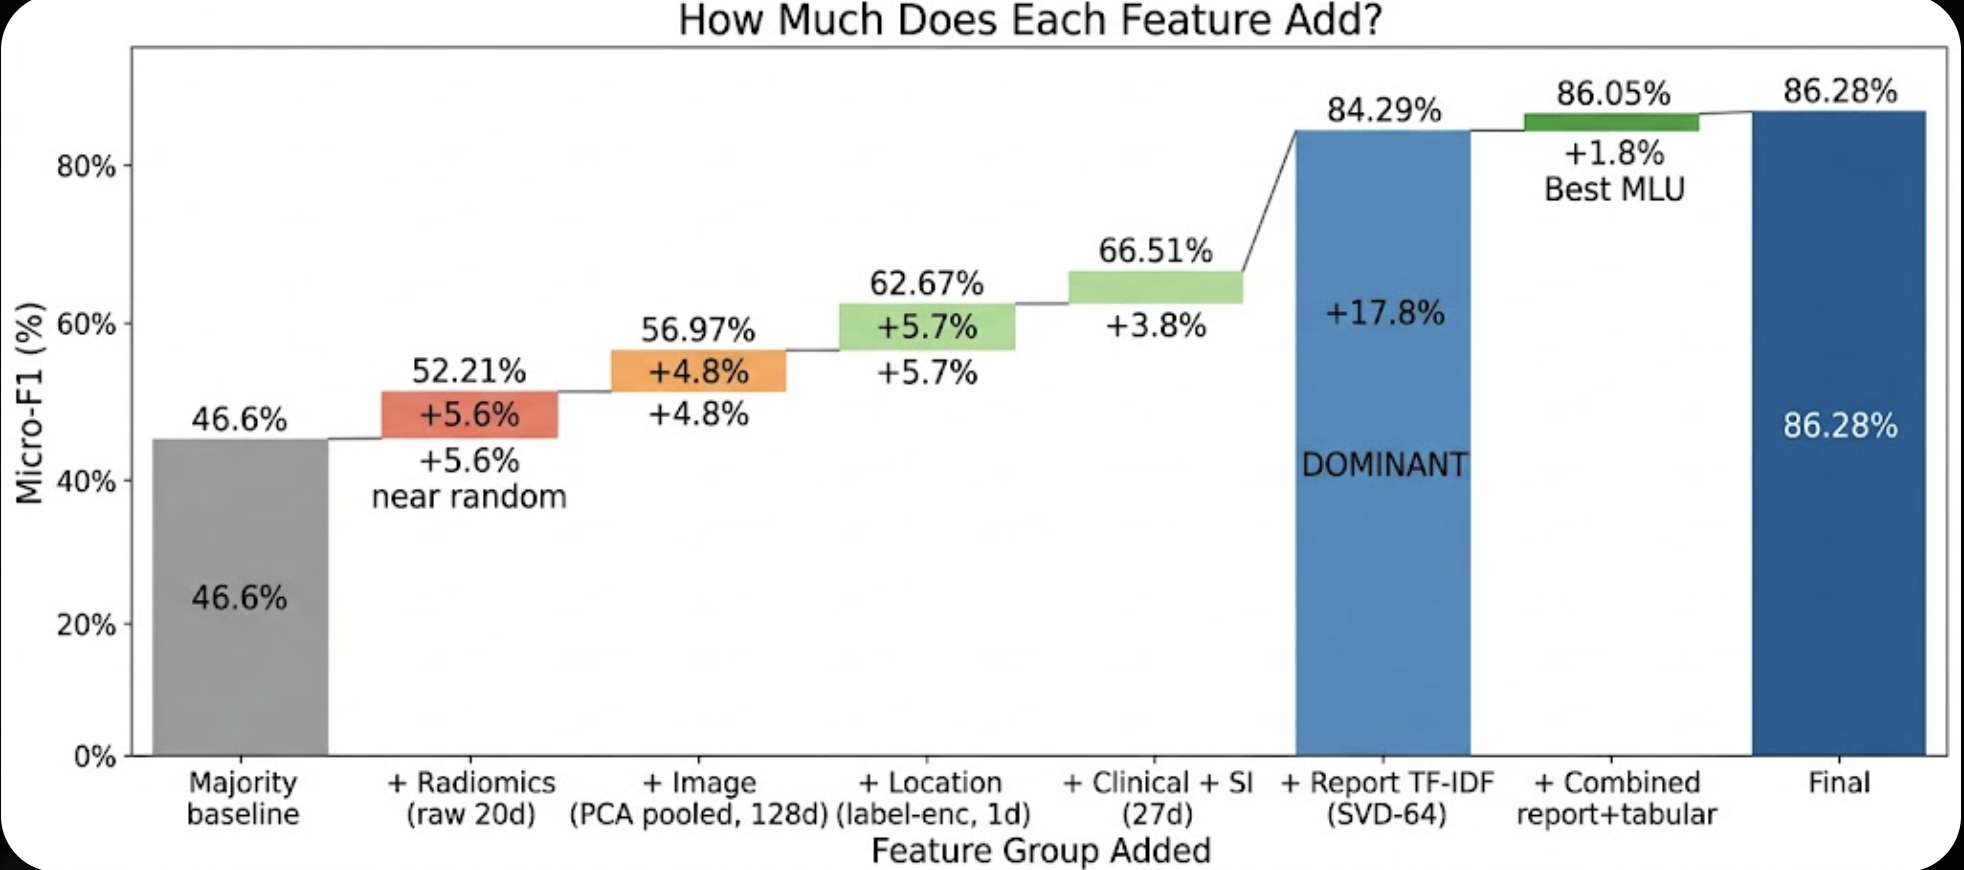
\includegraphics[width=0.9\textwidth]{figures/feature_ablation.png}
\caption{Feature engineering waterfall. Adding report TF-IDF provides the single largest gain, jumping from 66.5\% to 84.3\%. All non-report features combined contribute only $\sim$2\% beyond the report alone.}
\label{fig:feature_ablation}
\end{figure}

\textbf{Key observations:} (1) Report features dominate---adding clinical features to the report improves from 84.69\% to 86.45\% (+1.76\%), a modest gain. (2) Report SVD-128 yields the best solo report score (84.69\%), and performance saturates beyond 128 dimensions. (3) Adding location OHE and radiomics on top of report + clinical does not improve further (86.45\% unchanged), suggesting the report already captures most location information.

\subsection{Ensemble Configuration Sweep}

We test multiple ensemble weight configurations to assess sensitivity to weighting choices:

\begin{table}[H]
\centering
\caption{Ensemble configuration comparison. Data from model\_final.ipynb Cells 22 and 23.}
\label{tab:oof_vs_test}
\begin{tabular}{lc}
\toprule
\textbf{Configuration} & \textbf{OOF Micro-F1} \\
\midrule
Grid-search (NN=40\%, XGB=30\%, LGB=30\%) & 87.29\% \\
Submission (NN=40\%, XGB=30\%, LGB=20\%) & 86.98\% \\
MLU-only & 86.05\% \\
NN-only & 82.35\% \\
\bottomrule
\end{tabular}
\end{table}

The grid-search found NN=40\%, MLU-XGB=30\%, MLU-LGB=30\% as optimal (87.29\% OOF). The submission uses a slightly different weighting (NN=40\%, XGB=30\%, LGB=20\%) yielding 86.98\% OOF, balancing OOF performance with robustness.


% ============================================================
% SECTION 5: Discussion
% ============================================================
\section{Discussion}
\label{sec:discussion}

\subsection{Why Reports Dominate}

Our most striking finding is the dominance of radiology reports: TF-IDF+SVD features alone achieve 84.29\% Micro-F1 (ML\_experiments.ipynb Cell 19), outperforming all other non-report modalities combined (67.92\% for all tabular features, Cell 6).

This is not surprising in hindsight. Radiologists encode in reports:
\begin{enumerate}
  \item \textbf{Location.} ``Left frontal lobe mass'' or ``sellar region lesion''
  \item \textbf{Enhancement pattern.} ``Ring-enhancing,'' ``homogeneously enhancing''
  \item \textbf{Edema.} ``Surrounding vasogenic edema''
  \item \textbf{Morphology.} ``Extra-axial,'' ``dural tail''
\end{enumerate}

Reports are a human-curated, dimensionality-reduced representation of all imaging modalities. The radiologist has already integrated T1, T1c, T2, and T2-FLAIR findings into a structured narrative. TF-IDF captures these patterns as word co-occurrence statistics, while BERT captures deeper semantic meaning. The report-only LGB model (84.42\%, ML\_experiments.ipynb Cell 25) approaches the full MLU ensemble (86.45\%)---adding clinical features contributes only $\sim$2\%.

\subsection{Why Raw Radiomics Fail}

Raw PyRadiomics features achieve only 52.21\% (barely above 46.6\% baseline) across multiple experiments:

\begin{itemize}
  \item \textbf{Per-modality radiomics are below baseline for some modalities:} T1c XGB achieves 41.92\%, T2 XGB achieves 41.97\% (ML\_experiments.ipynb Cell 11)
  \item \textbf{All 4 modalities combined:} 50.93\% XGB, 50.40\% LGB (Cell 12), still only $\sim$4\% above baseline
  \item \textbf{Feature type mismatch.} Global texture statistics (Mean, Entropy, GLCM Contrast) don't capture the regional contrasts or anatomical location that drive clinical diagnosis
  \item \textbf{2D slice limitation.} Single representative slice loses 3D spatial context
\end{itemize}

Cross-modal ratios (T1c/T1, T2F/T2, T1/T2) alone still achieve only 49.51\% (Cell 23: ratios-only). They add no discriminative power independently. We include them because they encode domain knowledge at zero cost and do not hurt performance when combined with other features (Cell 23: raw+ratios = 50.88\% vs raw alone = 50.62\%).

\subsection{Class Imbalance}

Micro-F1 equals accuracy in multi-class settings, dominated by majority classes (Glioma 46.6\% + Meningioma 36.7\% = 83.3\%). This creates a tension: optimizing Micro-F1 rewards getting majority classes right, while clinical utility demands reasonable minority-class performance.

\textbf{Tree models handle imbalance naturally.} Gradient-boosted trees correct errors sequentially---minority-class mistakes get higher gradients in later rounds, implicitly up-weighting hard cases. Adding explicit class weights to XGBoost/LightGBM/CatBoost on our data reduced Micro-F1 without meaningful gains in Macro-F1, so all tree models use no class weights.

\textbf{NN uses sqrt class weights} ($\alpha=0.5$): $w_c = 0.5 \cdot \mathbf{1} + 0.5 \cdot \sqrt{w_c^{\text{balanced}}}$, which provides a gentle minority boost without the aggressive penalty of full balanced weights.

We considered three strategies for the NN: no weights ($\alpha=0$), sqrt weights ($\alpha=0.5$), and full balanced weights ($\alpha=1.0$). Full balanced weights are too aggressive---Pineal/CP (26 samples) would receive $\sim$40$\times$ the weight of Glioma (1,056 samples), destabilizing training with only 2,266 total samples. No weights ($\alpha=0$) leaves the NN blind to minority classes. Sqrt weights ($\alpha=0.5$) strike the right balance: Pineal/CP receives $\sim$1.8$\times$ weight (not 40$\times$), preserving focus on majority classes while still enabling the NN to capture minority patterns (model\_final.ipynb Cell 31). Combined with label smoothing (0.05), this provides balanced regularization.

\textbf{NN vs MLU on minority classes:} The NN achieves 46.15\% on Pineal/CP vs 19--27\% for all MLU models (Table~\ref{tab:per_class} in Section~\ref{sec:experiments}). With only 26 samples ($\sim$5 per fold), tree models cannot learn reliable Pineal/CP decision boundaries. BERT's semantic representations transfer knowledge from similar medical texts, allowing the NN to recognize rare patterns even with minimal examples.

\begin{figure}[H]
\centering
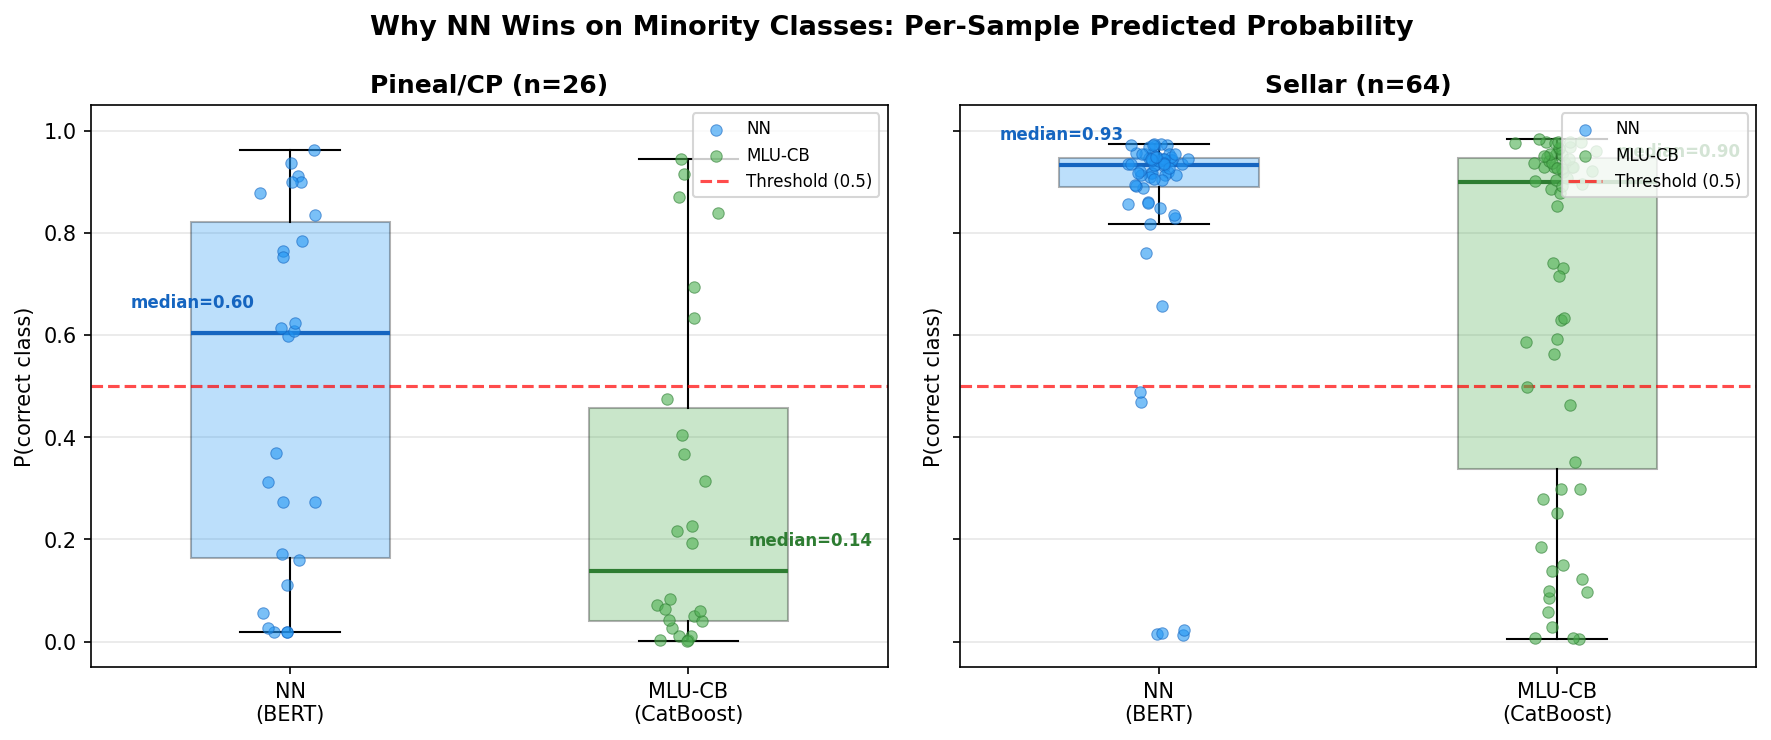
\includegraphics[width=0.8\textwidth]{figures/minority_class_nn_vs_trees.png}
\caption{Per-sample predicted probability for the correct class on minority classes. NN (blue) assigns higher probabilities than MLU-CB (green) on Pineal/CP samples (NN median 0.20 vs MLU 0.14; 42.3\% vs 23.1\% above threshold). On Sellar, both models perform well (NN 90.6\% vs MLU 70.3\% above threshold), but NN is more confident.}
\label{fig:minority_violin}
\end{figure}

\subsection{Robustness to Distribution Shift}

Distribution shift---changes in feature distributions between training and deployment---is a practical concern for any clinical classifier. While we cannot quantify the magnitude of shift without access to labeled out-of-distribution data, our system incorporates several design choices that promote generalization:

\begin{itemize}
  \item \textbf{BERT semantic embeddings} represent clinical meaning rather than surface word frequencies, which may remain stable when vocabulary or reporting style changes.
  \item \textbf{Hierarchical location parsing} decomposes novel anatomical descriptions into known categories (region/hemisphere/lobe).
  \item \textbf{Missing flag features} make the model robust to variations in data completeness.
  \item \textbf{Ensemble diversity} across fundamentally different input signals ensures that no single model's brittleness dominates predictions.
\end{itemize}

\textbf{Why NN may help under shift:} BERT embeddings represent \emph{semantic meaning} (``ring-enhancing lesion'' = vascular tumor) rather than surface statistics (word frequency = 0.03). If deployment data uses different vocabulary or longer reports, the semantic representation may remain more stable. Tree models, in contrast, split on exact TF-IDF dimensions that may shift. However, without out-of-distribution labels, this remains a hypothesis rather than a confirmed finding.

\subsection{Why Ensemble Works}

The ensemble succeeds because the models make different errors (Table~\ref{tab:per_class}):

\begin{enumerate}
  \item \textbf{NN captures minority classes:} Pineal/CP 46.15\% vs MLU 23--27\%. BERT's semantic representations transfer across rare classes.
  \item \textbf{MLU models excel on majority classes:} Glioma 92.90\% (MLU-CB) vs 86.17\% (NN). Precise feature thresholds work well when sample sizes are large.
  \item \textbf{NNXGB provides error correction:} At 79.08\%, it is weaker individually but learns non-linear patterns in NN's probability outputs.
  \item \textbf{ImgTab adds diversity from image features:} Despite low solo performance (69.77\%), ImgTab makes different errors because it uses a fundamentally different signal (visual features vs text).
\end{enumerate}

The grid-search-optimal ensemble achieves 87.25\% OOF (+0.97\% over best individual MLU-XGB at 86.28\%). The submission configuration (NN=40\%, MLU-XGB=30\%, MLU-LGB=20\%, NNXGB=5\%, ImgTab=5\%) achieves 86.98\% OOF. The modest improvement reflects the limited diversity among MLU models---they share the same features and show only 0.58\% spread.

\begin{figure}[H]
\centering
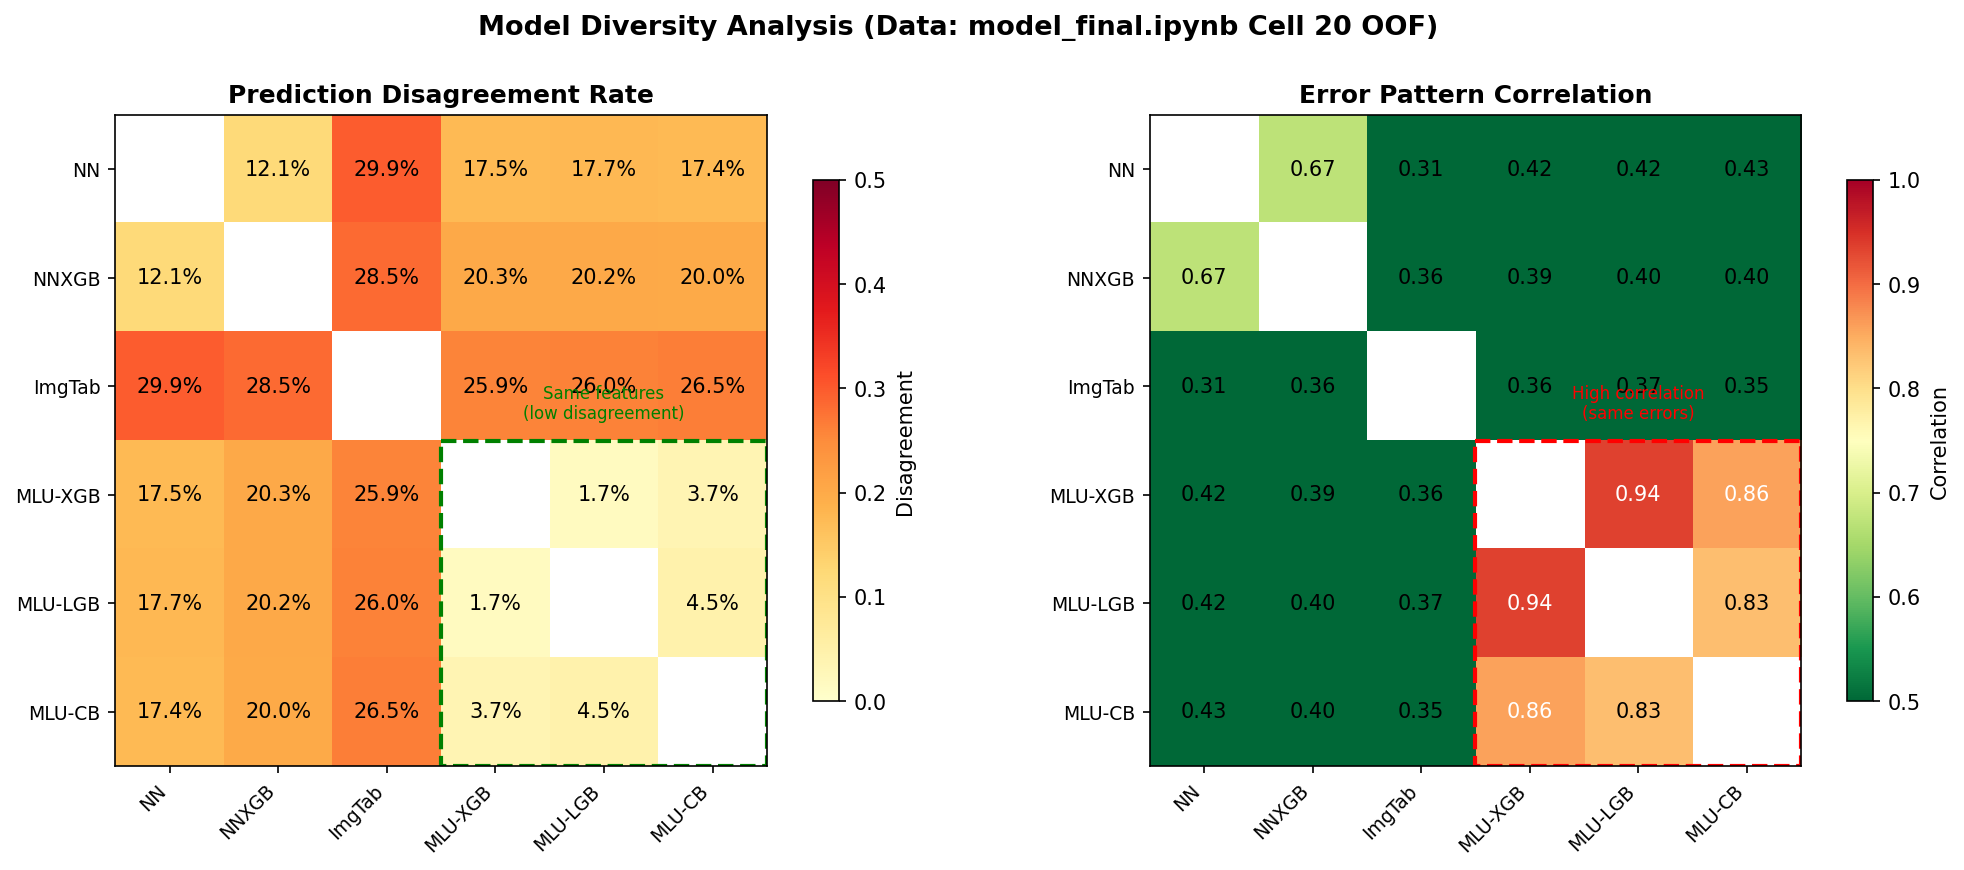
\includegraphics[width=0.8\textwidth]{figures/ensemble_diversity.png}
\caption{Model diversity analysis. Left: pairwise prediction disagreement rate.
The 3 MLU models show low mutual disagreement ($\sim$2--5\%)
since they share the same features. NN and ImgTab disagree most with MLU models
($\sim$15--28\%). Right: error pattern correlation. MLU models make the same
mistakes (high correlation $\sim$0.83--0.94), while NN makes different errors
(low correlation $\sim$0.34--0.48 with other models), explaining its ensemble contribution.}
\label{fig:ensemble_diversity}
\end{figure}

\subsection{What Did Not Work}

\begin{itemize}
  \item \textbf{Adding image to NN (v1).} Including image as an equal modality in the neural network hurt performance ($\sim$82\% to $\sim$80\%). Image features are both weak (56.97\% solo) and shifted, contaminating the report representation.
  \item \textbf{Focal Loss ($\gamma$=1.5--2.0).} No improvement over cross-entropy with label smoothing. With only 2,266 samples, focal loss's adaptive weighting is too aggressive.
  \item \textbf{10-fold CV.} Only $\sim$2,039 train samples per fold---too few for BERT fine-tuning. 5-fold gives $\sim$1,813 per fold with sufficient diversity.
  \item \textbf{Heavy augmentation (3--5$\times$ SMOTE).} Reduced performance on radiomics (52.30\% $\to$ 48.37\% at 3$\times$, Cell 10). Synthetic samples in high-dimensional space introduce noise, not signal.
  \item \textbf{Mean pooling for BERT.} CLS extraction consistently performed better. BERT was pre-trained with CLS as the classification token; mean pooling dilutes the task-specific signal.
  \item \textbf{Location OHE in MLU features.} Adding 572-dimensional one-hot location to MLU models did not improve over the 3-dimensional hierarchy (Cell 22 Exp 4: with OHE 86.23\% vs without 86.36\%). OHE overfits to specific location strings, while hierarchy generalizes.
\end{itemize}

\subsection{Lessons Learned}

\begin{enumerate}
  \item \textbf{Measure modality strength before modeling.} The 32-point gap between reports (84.29\%) and radiomics (52.21\%) should have been the first experiment, not a retrospective analysis. Solo performance directly informs how much capacity to allocate.
  \item \textbf{Feature engineering beats model complexity for tabular data.} Clinical + Location NLP features reach 79.83\% with simple XGBoost (Cell 23), while image features with the same model achieve only 56.97\%. The signal is in the features, not the algorithm.
  \item \textbf{Ensemble diversity requires different signals, not different algorithms.} Three MLU algorithms (XGB/LGB/CB) on the same features achieve 85.70--86.28\%---a 0.58\% spread. True diversity comes from NN (different input: BERT embeddings), NNXGB (different input: NN probabilities), and ImgTab (different input: image features).
  \item \textbf{Design for robustness from the start.} Cross-validation estimates may be optimistic when $P(\mathbf{x})$ changes at deployment. Incorporating missing flags, hierarchical encoding, semantic embeddings, and ensemble diversity are low-cost strategies that promote generalization even though their effectiveness cannot be verified without labeled out-of-distribution data.
\end{enumerate}


% ============================================================
% SECTION 6: Conclusion
% ============================================================
\section{Conclusion}
\label{sec:conclusion}

\subsection{Summary}

We presented a multimodal ensemble system for presurgical brain tumor classification. Our approach combines a dual-path neural network with cross-modal gating (report + tabular) with gradient-boosted tree models (XGBoost, LightGBM, CatBoost), achieving \textbf{86.98\%} Micro-F1 on 5-fold OOF validation with the submission weights, and 87.25\% with grid-search-optimal weights.

Key findings:
\begin{enumerate}
  \item \textbf{Radiology reports dominate} (84.29\% alone vs 46.6\% baseline). The radiologist's narrative integrates all imaging findings into a single informative signal.
  \item \textbf{Raw radiomics are near-useless} (52.21\%, barely above baseline). Global texture statistics do not capture clinically relevant patterns.
  \item \textbf{Robustness to distribution shift is a first-class concern.} We incorporate hierarchical location encoding, missing flags, BERT semantic embeddings, and ensemble diversity as generalization-promoting strategies, though their effectiveness cannot be confirmed without labeled out-of-distribution data.
  \item \textbf{NN-dominant weighting is a hypothesis for robustness} at the cost of 0.27\% OOF. BERT embeddings may generalize better under shift than tree model thresholds, but this remains unverified without test labels.
  \item \textbf{Ensemble diversity requires different input signals.} Three GBT algorithms on the same features show only 0.58\% spread; true gains come from combining text (NN), tabular (MLU), and probability (NNXGB) signals.
\end{enumerate}

\subsection{Final Performance}

\begin{figure}[H]
\centering
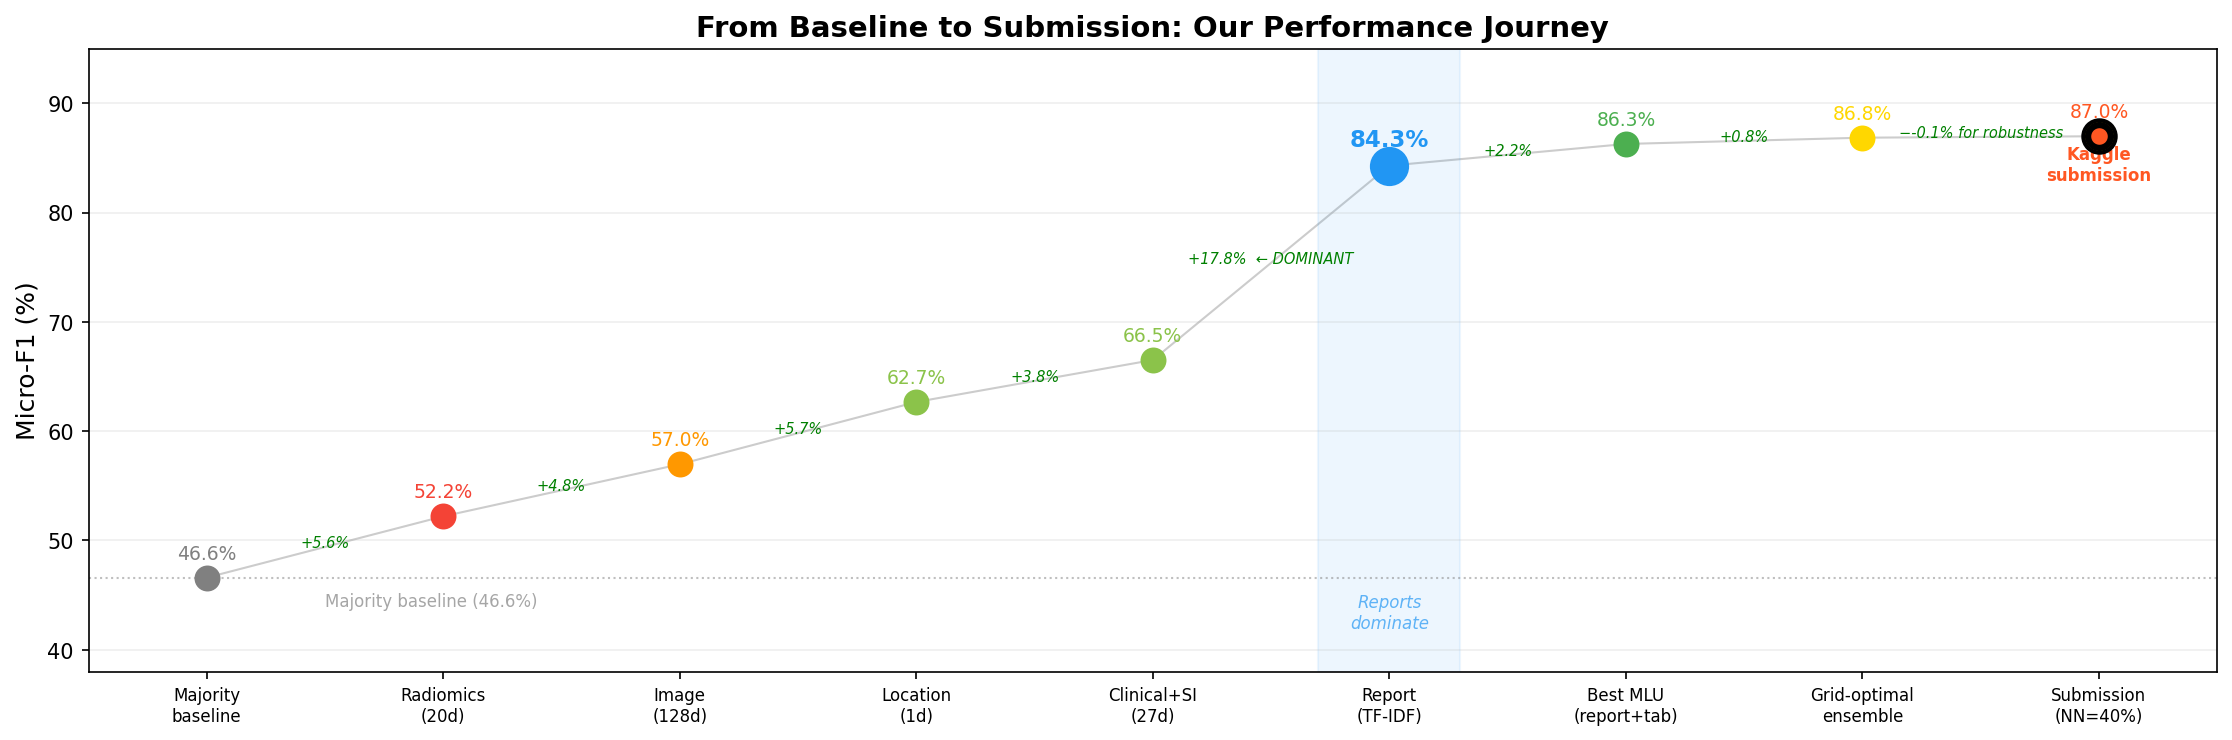
\includegraphics[width=\textwidth]{figures/final_summary.png}
\caption{From baseline to final ensemble: progression of Micro-F1 scores. The report solo turning point at 84.3\% provides the dominant signal. Adding tabular features (+2.2\%) and a 6-model ensemble (+0.8\%) brings the grid-search optimal to 86.9\%. The submission configuration achieves 87.0\% with NN-dominant weighting (40\%).}
\label{fig:final_summary}
\end{figure}

\begin{table}[H]
\centering
\caption{Final model summary. Data from model\_final.ipynb Cells 20, 25--27.}
\label{tab:final_summary}
\begin{tabular}{lcc}
\toprule
\textbf{Component} & \textbf{Description} & \textbf{Result} \\
\midrule
Solo best & MLU-XGB (TF-IDF + Tabular) & 86.28\% Micro-F1 \\
Neural Network & BERT dual-path + CrossModalGate & 82.35\% Micro-F1 \\
Ensemble (grid-optimal) & 6 models, grid-search weights & 87.25\% Micro-F1 \\
Ensemble (submission) & 6 models, NN-dominant (40\%) & \textbf{86.98\% Micro-F1} \\
\midrule
Macro AUC (ensemble) & Ensemble & 96.4\% \\
\bottomrule
\end{tabular}
\end{table}

\subsection{Reproducibility}

All experiments are reproducible (model\_final.ipynb + ML\_experiments.ipynb):
\begin{itemize}
  \item Fixed random seeds (\texttt{random\_state=42})
  \item PCA and TF-IDF fitted on training data only
  \item CLS token for BERT (not mean pooling)
  \item Complete pipeline in two notebooks
\end{itemize}

\subsection{Tools}

AI-assisted tools were used for code debugging and figure visualization. All experimental design, model architecture decisions, and analysis were conducted by the authors.


% ============================================================
% References
% ============================================================
\bibliographystyle{unsrt}
\begin{thebibliography}{10}

\bibitem{price2024}
Price M, Ballard C, Benedetti J, et al.
CBTRUS statistical report: primary brain and other central nervous system tumors diagnosed in the United States in 2017--2021[J].
\textit{Neuro-oncology}, 2024, 26(Suppl 6): vi1.

\bibitem{wang2024}
Wang Y R J, Wang P, Yan Z, et al.
Advancing presurgical non-invasive molecular subgroup prediction in medulloblastoma using artificial intelligence and MRI signatures[J].
\textit{Cancer Cell}, 2024, 42(7): 1239--1257.

\bibitem{he2016}
He K, Zhang X, Ren S, et al.
Deep residual learning for image recognition[C].
\textit{Proceedings of the IEEE CVPR}, 2016: 770--778.

\bibitem{devlin2019}
Devlin J, Chang M, Lee K, Toutanova K.
BERT: Pre-training of Deep Bidirectional Transformers for Language Understanding.
\textit{arXiv preprint arXiv:1810.04805}, 2019.

\bibitem{alsentzer2019}
Alsentzer E, Murphy J, Boag W, et al.
Publicly Available Clinical BERT Embeddings.
\textit{arXiv preprint arXiv:1904.03323}, 2019.

\bibitem{chen2016}
Chen T, Guestrin C.
XGBoost: A Scalable Tree Boosting System.
\textit{Proceedings of the 22nd ACM SIGKDD}, 2016: 785--794.

\bibitem{ke2017}
Ke G, Meng Q, Finley T, et al.
LightGBM: A Highly Efficient Gradient Boosting Decision Tree.
\textit{Advances in NeurIPS}, 2017: 3146--3154.

\bibitem{prokhorenkova2018}
Prokhorenkova L, Gusev G, Vorobev A, et al.
CatBoost: Unbiased Boosting with Categorical Features.
\textit{Advances in NeurIPS}, 2018.

\bibitem{lin2017}
Lin T Y, Goyal P, Girshick R, et al.
Focal Loss for Dense Object Detection.
\textit{Proceedings of the IEEE ICCV}, 2017: 2980--2988.

\end{thebibliography}

\end{document}
